%% Springer Nature submission, single-column. For the official class, open
%% the Springer Nature template on Overleaf and replace the preamble with
%% \documentclass[pdflatex,sn-mathphys-num]{sn-jnl}; the section files and
%% refs.bib need no changes.
\documentclass[12pt]{article}
\usepackage[a4paper,margin=1in]{geometry}
\usepackage[T1]{fontenc}
\usepackage{lmodern}
\usepackage{microtype}
\usepackage{amsmath,amssymb,graphicx,booktabs,url,setspace}
\usepackage[table]{xcolor}
\usepackage{tikz}
\usetikzlibrary{positioning,arrows.meta,fit,calc}
\usepackage[hidelinks]{hyperref}
\usepackage[numbers,sort&compress]{natbib}
\onehalfspacing
\bibliographystyle{unsrtnat}
\graphicspath{{figures/}}

\title{\textbf{Evidence Coverage and the Cost of False Isolation: Verifying
Malicious Beacon Nodes in Mobile Ad Hoc Networks}}
\author{%
  \normalsize Amruth V\,$^{1,\ast}$ \quad Devaraj Verma C\,$^{1}$ \\[8pt]
  \small $^{1}$Department of Computer Science and Engineering, \\
  \small JAIN (Deemed-to-be University), Bengaluru 562112, Karnataka, India \\[6pt]
  \small $^{\ast}$Corresponding author: Amruth V, Research Scholar \\
  \small \texttt{amruthv020@gmail.com}%
}
\date{}

\begin{document}
\maketitle

\begin{abstract}
\noindent Malicious beacon nodes corrupt the position estimates of nodes that
never exchange traffic with them. Prior defences detect them from
localisation evidence and remove them permanently; we study the decision
that precedes removal and what an error costs, over 525 distinct ns-3
simulations. First, coverage: every detector restricted to one evidence
class, including re-implemented localisation-only and behaviour-only
baselines from the literature, confirmed the attack outside that class in at
most 3 of 30 seeds, while collecting both classes confirmed every attacker.
Second, we introduce cumulative false isolation~$\Phi$, in node-seconds.
Isolating only on confirmation withdrew 3.9--5.0\% of honest-beacon service
against 74.8\% for the strongest immediate-isolation policy, and the gap held
when the schedules were enforced. Enforcement also showed that releasing a
beacon when its verdict clears re-admits forwarding attackers, whose
behavioural evidence vanishes while isolated; releasing only when that
evidence returns prevented every re-admission. Third, every weighted
Stouffer detector can confirm attackers that neither branch confirms alone,
but an attack scaled in intensity reaches that region only if the branches'
detection thresholds lie within a factor of $1+\sqrt{2}$. The condition
explains a negative result: for these attacks, a calibrated disjunction of
the two baselines matched our fused pipeline's coverage and false isolation
and confirmed attackers as fast or faster, most clearly under 4--8\,dB
shadowing. Results cover one dense 25-node topology.

\medskip
\noindent\textbf{Keywords} Mobile ad hoc networks $\cdot$ Beacon nodes
$\cdot$ Trust management $\cdot$ Evidence fusion $\cdot$ Node isolation
$\cdot$ Localisation security
\end{abstract}

\section{Introduction}

Mobile ad hoc networks (MANETs) operate without fixed infrastructure. Nodes
organise themselves, forward one another's traffic, and reconfigure as the
topology changes. The properties that make this attractive for disaster
response, defence communication and location-aware services are the same
ones that make the network hard to secure. There is no central authority to
consult, no stable membership, and no reliable way to tell a node that is
failing from a node that is lying.

Beacon nodes deserve separate treatment within this problem. A beacon
advertises position information that neighbouring nodes consume to
localise themselves. A compromised beacon therefore corrupts the position
estimates of nodes it never exchanged data traffic with, and the corruption
propagates through the localisation computation, not through the
routing fabric. The consequences differ in kind from ordinary
packet-dropping attacks, not merely in degree. A node that drops packets
degrades a service the network can measure; a beacon that lies about its
position degrades a service the network has no independent way to check.

Elimination of malicious beacons from localisation evidence is well studied
for static beacons. Liu, Ning and Du detect a beacon whose RSSI-implied
distance disagrees with the distance implied by its declared position, and
revoke it once enough alerts accumulate~\cite{liu2005detecting}. Kuriakose
et al.~\cite{kuriakose2023embn} address the same problem in EMBN-MANET, a
UWB-based mobile ad hoc network, using RSSI and trilateration residuals, and
report complete identification when fewer than four malicious beacons share
a neighbourhood. Both establish that detection from localisation evidence is
tractable. What neither settles is the decision that precedes removal, and
what happens to the network when that decision is wrong: revocation in both
is permanent.

Both questions matter for a practical reason. In a mobile wireless
environment, congestion, transient link failure, interference and mobility
all produce observations that resemble attack. A verification stage
separating detection from confirmation therefore has a plausible role, a
need also identified in work on trust change and revision~\cite{chatzidakis2022trust}
and on verification supported by observable evidence~\cite{li2019dapv,ryu2023reputation}.
Because a removed beacon is a beacon whose localisation service is lost
to its neighbours, removal is not free: a verification mechanism that is too
eager degrades exactly the service it exists to protect.

\subsection{Problem statement}

The paper addresses four questions. The first is whether a detector that
uses one class of evidence can confirm beacons whose attack leaves no
signature in that class, and whether collecting both behavioural and
localisation evidence closes the gap (Sections~\ref{sec:coverage},
\ref{sec:baselines}, \ref{sec:sparse} and~\ref{sec:scale}). The second is how
much honest-beacon service isolation policies withdraw, and how waiting for
confirmation changes that cost (Sections~\ref{sec:policy}
and~\ref{sec:phi}). The third is whether an isolated beacon can be released
safely once the evidence against it clears (Section~\ref{sec:release}). The
fourth is when fused evidence can confirm an attacker that neither branch
confirms alone, and whether a fused detector is better than classical
single-evidence detectors run side by side (Sections~\ref{sec:region},
\ref{sec:sweep}, \ref{sec:baselines}, \ref{sec:sparse} and~\ref{sec:scale}).

\subsection{Contributions}

We answer these questions in ns-3 across 780 simulation runs: a 30-seed
detection campaign over three attack scenarios and a clean network, six
isolation policies replayed over that campaign and checked by enforcing them
in the simulator, an iterated closed loop, two attack-intensity sweeps,
log-normal shadowing, a sparse topology, a 50-node network with two
simultaneous attackers, and two re-implemented literature baselines evaluated
on the same traces.

\begin{enumerate}
\item \textbf{Evidence coverage.} We frame malicious-beacon
      verification as a question of evidence coverage rather than detection
      accuracy. Every detector restricted to one evidence class, including
      re-implemented localisation-only and behaviour-only baselines from the
      literature, was blind to the attack outside that class, in the small,
      sparse and 50-node networks alike; collecting both classes confirmed
      the attacker in 209 of 210 attacked runs of the dense network and
      both attackers in every run at 50 nodes. The verification pipeline that
      fuses the two classes into per-observer trust and a three-state verdict
      is built from established components and is the vehicle for
      the study.

\item \textbf{A measure of what false isolation costs.} We introduce
      cumulative false isolation~$\Phi$, in node-seconds, and its normalised
      form~$\bar\Phi$, as complements to the false-positive rate, which says
      nothing about how long an error persists. Isolating only on
      confirmation withdrew 3.9--5.0\% of honest-beacon service on a clean
      network against 74.8\% for the strongest immediate-isolation policy,
      and the gap held when the schedules were enforced in the simulator,
      under shadowing and at 50 nodes.

\item \textbf{Release is as consequential as isolation.} Timed
      redemption is known to let attackers back in~\cite{bansal2003ocean,sen2010survey}.
      We show that release is unsafe even without a timer or any action by
      the attacker: releasing an isolated beacon when its verdict clears
      re-admits forwarding attackers in a closed loop, because isolation
      removes the very traffic their behavioural evidence comes from. An evidence-aware release rule
      prevented every re-admission at a small cost in false isolation, and
      showed that the advantage of confirmation-gated isolation comes from
      the gating itself.

\item \textbf{When fusion helps.} Every weighted Stouffer
      detector has a fusion-only region, containing attackers whose two anomalies are
      each sub-threshold and of comparable size, and an attack family scaled
      in intensity passes through it only if the branches' detection
      thresholds for that family lie within a factor of
      $1+\sqrt{2}\approx 2.414$. We offer this as an explanatory tool rather
      than a new result in fusion theory. The condition is checkable before any
      fusion experiment and predicted the outcome of two intensity sweeps.
      We also make explicit, for trust fusion, the calibration requirement on
      which any such test depends~\cite{stouffer1949,whitlock2005weighted}.

\item \textbf{Comparison with classical detectors.} In the
      small dense network a calibrated disjunction of the two literature
      baselines matched the fused pipeline's coverage and false isolation
      and confirmed attackers as fast or faster, as the fusion condition
      predicts. In the sparse and 50-node networks the same disjunction
      withdrew 11--24\% of honest-beacon service on a clean network against
      0--3\% for the pipeline. The pipeline's single-branch results show
      why: in the sparse network its peer-relative scoring of behaviour
      avoided the false alarms, and at 50 nodes fusion suppressed false
      alarms raised by its own behavioural branch. Fusion thus trades
      sensitivity near the threshold for fewer false isolations. In the
      sparse network the pipeline paid for this by confirming the
      forwarding attacker in only 4 of 10 seeds.

\item \textbf{Bounding results.} Localisation error
      (Appendix~\ref{sec:locerr}) shows that the two
      attack classes are disjoint in both evidence directions; detection and
      the false-isolation result survive 4 and 8\,dB shadowing at a cost in
      latency for forwarding attacks; and we report two negative results:
      the trust aggregation stage changed no verdict
      (Appendix~\ref{sec:ablation}), and neither isolation policy produced a
      throughput advantage surviving its confidence interval
      (Section~\ref{sec:policy}).
\end{enumerate}

\subsection{Organisation}

Section~\ref{sec:related} positions the work against the closest prior art.
Section~\ref{sec:model} defines the network and threat models.
Section~\ref{sec:framework} develops the model in full.
Section~\ref{sec:method} describes the simulation campaign.
Section~\ref{sec:results} reports results, Section~\ref{sec:discussion}
interprets them, Section~\ref{sec:threats} states threats to validity, and
Section~\ref{sec:conclusion} concludes. Appendix~\ref{sec:appendix}
reports secondary results.

\section{Related Work}
\label{sec:related}

\subsection{Trust-based detection and routing}

Trust management in MANETs has developed along two largely separate lines.
The first evaluates node reliability from forwarding behaviour, reputation
and recommendation, and uses the resulting score to steer route
selection~\cite{cai2019evolutionary,xia2013trust,sirajuddin2021tbsmr,singh2020self}.
Approaches in this line combine direct observation with neighbour
recommendation~\cite{singh2020self,sanchez2015model} and, more recently,
with learned models~\cite{dhand2025secure,mahamune2024trust}. The recurring
design questions are how to weight one's own observations against those of
others, how to age evidence, and how to resist a recommender that lies.

Three design axes recur. The first is what the trust score is computed
from. Early work used packet-forwarding ratio and drop
behaviour~\cite{xia2013trust,sanchez2015model}. Later schemes added energy,
mobility and link stability~\cite{veeraiah2021trust,thirunavukkarasu2022cluster},
and recent ones learn the score from features using gradient boosting or
neural models~\cite{ryu2023reputation,dhand2025secure}. The second is what
the score is used for. Most schemes feed it into route selection, either by
penalising low-trust hops in a single-path
protocol~\cite{pathan2018efficient,pari2023enhanced} or by distributing
traffic across trust-weighted multiple
paths~\cite{sirajuddin2021tbsmr,srilakshmi2021improved,srilakshmi2022secure}.
A smaller group treats trust as an admission-control question,
authenticating or excluding nodes before they
participate~\cite{tu2021active,lwin2020blockchain}. The third is how
recommendations from other nodes are weighted and filtered, since a
recommender may itself be
adversarial~\cite{singh2020self,rajeswari2021efficient,pari2023hybrid}.

Our work sits in the second and third of these but differs in what it
optimises. Almost all of the above evaluate the trust mechanism by its
effect on delivery ratio, throughput and delay, which measures the benefit
of excluding attackers. Far fewer measure the cost of excluding honest nodes
by mistake, and fewer still measure how long such an exclusion persists.
Schemes that also address energy and route
stability~\cite{thirunavukkarasu2022cluster,ponguwala2019e2sr} make the cost
side explicit for energy but not for availability. We argue in
Section~\ref{sec:framework} that a cumulative false-isolation measure
belongs alongside the false-positive rate, and Section~\ref{sec:results}
shows the two can differ by more than an order of magnitude for the same
detector.

A consistent finding across this line is that static thresholds produce
false positives under changing topology, which motivates dynamic or adaptive
trust state. Chatzidakis and Hadjiefthymiades~\cite{chatzidakis2022trust}
make this explicit, proposing a mechanism that identifies malicious nodes,
alerts the network, and subsequently restores trust when a node resumes
healthy behaviour or when an earlier classification proves incorrect. The
possibility of restoration is important and we adopt it: a verification
scheme that can only ever remove nodes accumulates errors monotonically, a
point our clean-network experiment makes quantitatively in
Section~\ref{sec:phi}.

\subsection{Learned trust models}

A recent line of work replaces hand-specified trust arithmetic with learned
models. Gradient-boosted trees have been applied to trust-value estimation
for malicious node detection~\cite{dhand2025secure}, feature-optimisation and
classification pipelines to intruder isolation~\cite{kavitha2019india}, and
reinforcement learning to reputation-driven route
selection~\cite{ryu2023reputation}. The attraction is that the decision
boundary is fitted rather than assumed, which matters when the relationship
between evidence and misbehaviour is not monotone or not separable by a
threshold.

The coverage failure reported in Section~\ref{sec:results} is not, however,
a modelling failure. Under the false-location attack the delivered-throughput
trace is identical to the clean-network trace in every seed, so the
behavioural evidence stream contains no information about the attack. No
estimator recovers signal from an identical trace, and a learned model
restricted to that evidence class would fail exactly as the statistical one
does. Evidence coverage is a property of what is collected, not of how it is
combined. A learned rule could contribute at the combination stage; it
cannot address a limitation upstream of it.

\subsection{Localisation-centred beacon security}

The second line is beacon-specific, using ranging measurements and geometric
consistency to determine whether an advertised position is
plausible~\cite{kuriakose2023embn,liu2008attack}. Robustness here usually
means tolerating a bounded number of lying beacons rather than identifying
them individually, and the classical results bound achievable localisation
error as a function of the fraction of compromised anchors.

Secure localisation has a longer history in sensor networks. SeRLoc bounds a
node's position using directional beacons without range
measurements~\cite{lazos2004serloc}; verifiable multilateration rejects
position claims inconsistent with distance bounds~\cite{capkun2006secure};
and Liu, Ning and Du detect malicious beacons by the inconsistency between
measured and declared range, revoking a beacon once a base station has
received enough independent alerts~\cite{liu2005detecting}. Our localisation
branch uses the same residual as the last of these. What differs is the
setting --- mobile beacons and commodity 802.11 RSSI rather than static
beacons or UWB ranging --- and the decision rule: our confirmation is
reversible, and we measure what a false confirmation costs while it
persists.

The two lines overlap less than their subject matter suggests, and the gap
is visible in the evaluations rather than in the methods: a trust-routing
paper does not typically test an attacker whose only misbehaviour is
positional, and a beacon-security paper does not typically test one whose
only misbehaviour is in forwarding. This is an observation about the papers
we surveyed, not a systematic survey finding.

\subsection{EMBN-MANET}

EMBN-MANET~\cite{kuriakose2023embn} is the recent work closest to ours. Its
detection evidence consists of RSSI measurements and trilateration in a
UWB-based mobile ad hoc network. A $k$-polytopes procedure identifies
centroids, from which an identifier infers suspicious activity, and a valid
probable location $T_{loc}$ is compared against the location $F_{loc}$ a
suspect beacon shares during coordinated localisation. Its threat model is a
beacon that masquerades or spoofs by providing false location coordinates.
Its response is to assign a reputation value to the identified beacon and to
exclude it from coordinating localisation once that value crosses a
threshold. Reported identification is complete when fewer than four
malicious beacons occupy a neighbourhood and exceeds 85\% above that count.
The authors state that their work addresses static beacon nodes and name
detection for mobile beacons as future work.

Four differences follow. First, EMBN-MANET's evidence is entirely
localisation-derived. A beacon that advertises correct coordinates while
selectively dropping transit traffic falls outside what its measurements can
observe, and outside the threat model it sets out to address. Second, its
response excludes a beacon from localisation coordination. It does not
remove the node from packet forwarding, so it makes no claim about
post-removal route continuity or throughput, and it is not a model of the
forwarding-level isolation we evaluate. None of our isolation policies is an
implementation of its response. Third, its beacons are static and ours are
mobile, which its authors identify as the natural extension. Fourth, its
accuracy figure is conditional on attacker density within a neighbourhood,
and we quote it as such.

\begin{table}[!t]
\caption{Evidence classes and observable attack surface by approach family.
Entries are read from published descriptions, not measured.}
\label{tab:families}
\centering
\small
\begin{tabular}{@{}lccccc@{}}
\toprule
Approach & Loc.\ evid. & Beh.\ evid. & Rec.\ trust & Mob.\ beac. & FI metric \\
\midrule
Localisation-centred~\cite{kuriakose2023embn,liu2005detecting,liu2008attack} & \checkmark & & & & \\
Behavioural trust~\cite{xia2013trust,sanchez2015model} & & \checkmark & \checkmark & \checkmark & \\
Multipath trust~\cite{sirajuddin2021tbsmr,srilakshmi2021improved} & & \checkmark & \checkmark & \checkmark & \\
Learned trust~\cite{ryu2023reputation,dhand2025secure} & & \checkmark & & \checkmark & \\
Admission control~\cite{tu2021active,lwin2020blockchain} & & \checkmark & \checkmark & \checkmark & \\
This work & \checkmark & \checkmark & \checkmark & \checkmark & \checkmark \\
\bottomrule
\end{tabular}
\par\smallskip\footnotesize
Loc./Beh.\ evid.: localisation and behavioural evidence. Rec.\ trust:
recommendation-based trust. Mob.\ beac.: mobile beacons. FI metric: reports
a false-isolation cost measure.
\end{table}

\subsection{Structured comparison and basis for comparison}

Because we decline a numerical accuracy comparison, we give a structured
qualitative one instead. Table~\ref{tab:families} states, for each family of
approach, which evidence classes it observes and which attack classes
therefore fall inside its scope. Localisation-centred beacon security
observes the evidence class that the false-location attack disturbs and not
the class that selective forwarding disturbs; behavioural trust schemes
observe the converse. Our contribution is not a better detector within
either column but the observation that the columns are disjoint and that a
beacon can misbehave in whichever one is not being watched. The final column
is the metric introduced in Section~\ref{sec:framework}; we are not aware of
prior work in this area that reports the persistence of false exclusions
rather than their rate, though we offer that as a gap in our reading, not an
exhaustive search.

Reported detection accuracy in this field is conditioned on an attack model,
a topology, a mobility regime, a traffic load and an attacker density, all
of which vary across papers. It also saturates: when published figures
cluster between 90\% and 99\%, a difference of one percentage point carries
less information than the differences in evaluation conditions that
produced it. Our own results show why. Every configuration tested, including
both single-evidence ones, achieves perfect recall against the attack its
evidence can observe and near zero against the attack it cannot. An accuracy
figure drawn from the first case alone would be correct and uninformative.
The informative axis is coverage, and we compare against EMBN-MANET on it,
where the comparison is both fair and decidable.

\section{Network and Threat Model}
\label{sec:model}

\subsection{Network model}

The network is a dynamic graph $G(t) = (V, E(t))$ over $N$ mobile nodes with
time-varying wireless links. A subset $\mathcal{B} \subseteq V$ consists of beacon
nodes advertising position information usable by neighbours for
localisation. A subset $\mathcal{B}_m \subseteq \mathcal{B}$ is compromised.
Each monitored beacon $i$ carries a state
\begin{equation}
\label{eq:state}
S_i(t) \in \{\textsc{Normal}, \textsc{Suspicious}, \textsc{Confirmed}\}.
\end{equation}
The intermediate state exists so that a single anomalous observation does
not directly authorise removal.

The pipeline both raises suspicion and decides what to do about it; our
contribution concerns the second step, verification and response. Attackers are insiders
holding valid credentials, so cryptographic authentication does not resolve
the problem: an authenticated node can still lie.

\subsection{Attack model}

We evaluate three attacker behaviours, chosen so the first two are disjoint
in the evidence they disturb and the third combines them.

\textbf{A1, false location.} The compromised beacon advertises a position
displaced from its true position, while forwarding all transit traffic
honestly. This corrupts localisation and, by construction, produces no
forwarding anomaly. The offset $\delta$ is applied to both coordinates and
the result is clamped to the field,
\begin{equation}
\label{eq:clamp}
x^{c} = \min\bigl(X, \max(0, x + \delta)\bigr), \qquad
y^{c} = \min\bigl(Y, \max(0, y + \delta)\bigr).
\end{equation}
An unclamped beacon is therefore displaced by $\delta\sqrt{2} = 424$\,m for
$\delta = 300$\,m, while one near the far corner is displaced much less.
Over the campaign the realised displacement averaged 267\,m, with median
271\,m and 95th percentile 299\,m (Section~\ref{sec:locerr}). We report the
measured displacement alongside the nominal parameter, since the effective
attack strength depends on where in the field the attacker happens to be.

\textbf{A2, selective forwarding.} The compromised beacon advertises its true
position and drops transit packets with probability $p$. This degrades
delivery and produces no localisation anomaly.

\textbf{A3, hybrid at half intensity.} The compromised beacon applies both
behaviours with each halved: offset $\delta/2$ and drop probability $p/2$.

The choice to halve rather than compound is deliberate. Compounding both
behaviours at full strength produces an attacker that is more conspicuous on
every axis at once, which tests nothing A1 and A2 do not already test.
Halving produces an attacker that is less conspicuous on each axis while
remaining malicious on both. That is the configuration under which a fusion
advantage, if the mechanism confers one, should appear, because each
single-evidence branch operates closer to its detection threshold. A3 is
therefore a test of the fusion hypothesis and not a demonstration of it,
and Section~\ref{sec:sweep} sweeps its intensity.

\begin{table}[!t]
\caption{Principal notation.}
\label{tab:notation}
\centering
\small
\begin{tabular}{@{}ll@{}}
\toprule
Symbol & Meaning \\
\midrule
$FR_i(t)$ & forwarding ratio of beacon $i$ \\
$z_B, z_L$ & standardised behavioural / localisation evidence \\
$A_B, A_L$ & oriented anomaly scores \\
$Z_{ij}(w)$ & fused evidence statistic \\
$T^D, T^I, T^H$ & direct, indirect, historical trust \\
$\hat C_i(t)$ & collapsed confidence \\
$\tau_N, \tau_M$ & normal and malicious thresholds \\
$W, K$ & persistence window and confirmation count \\
$\mathcal{B}_{iso}(t)$ & isolation set \\
$\theta_B, \theta_L$ & branch detection thresholds in attack intensity \\
$R_{TH}$ & throughput recovery ratio \\
$\Phi, \bar\Phi$ & cumulative false isolation (node-seconds) and its normalised form \\
\bottomrule
\end{tabular}
\end{table}

\section{Proposed Framework}
\label{sec:framework}

This section develops the verification and recovery model in full.
Fig.~\ref{fig:pipeline} shows how the pieces connect; notation is summarised
in Table~\ref{tab:notation}.

\begin{figure}[!t]
\centering
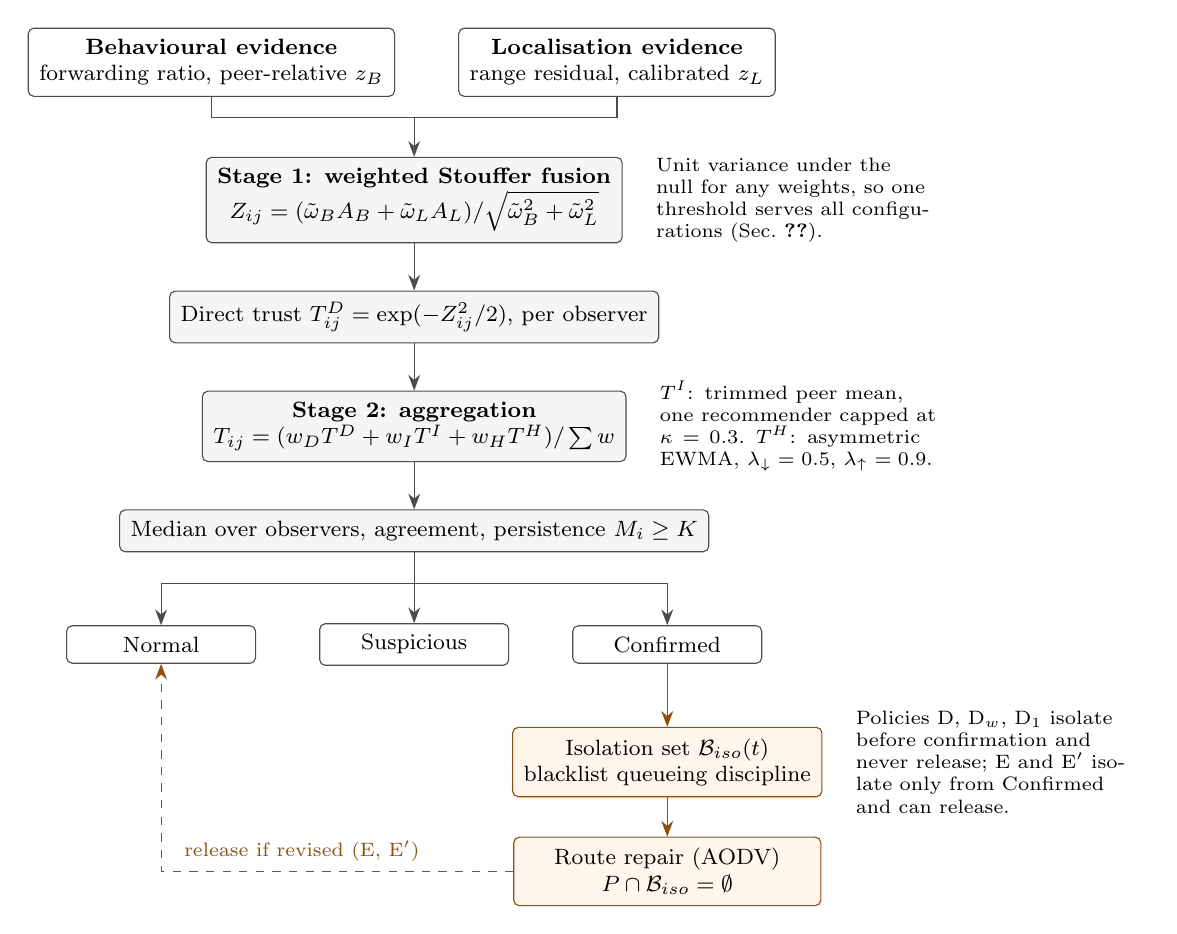
\begin{tikzpicture}[
  font=\footnotesize,
  box/.style={draw=black!70, rounded corners=2pt, align=center, fill=gray!8,
              minimum width=4.6cm, inner sep=4pt},
  ev/.style={box, fill=white, minimum width=3.6cm},
  st/.style={draw=black!70, rounded corners=2pt, minimum width=2.4cm,
             inner sep=4pt, fill=white},
  iso/.style={box, fill=orange!8, draw=orange!60!black, minimum width=3.9cm},
  note/.style={align=left, font=\scriptsize, text width=3.6cm},
  arr/.style={-{Stealth[length=2mm]}, black!70},
  node distance=6mm]
\node[ev] (beh) {\textbf{Behavioural evidence}\\forwarding ratio, peer-relative $z_B$};
\node[ev, right=8mm of beh] (loc) {\textbf{Localisation evidence}\\range residual, calibrated $z_L$};
\node[box, below=12mm of $(beh)!0.5!(loc)$] (s1) {\textbf{Stage 1: weighted Stouffer fusion}\\
  $Z_{ij}=(\tilde\omega_B A_B+\tilde\omega_L A_L)/\sqrt{\tilde\omega_B^2+\tilde\omega_L^2}$};
\node[box, below=of s1] (td) {Direct trust $T^D_{ij}=\exp(-Z_{ij}^2/2)$, per observer};
\node[box, below=of td] (s2) {\textbf{Stage 2: aggregation}\\
  $T_{ij}=(w_D T^D+w_I T^I+w_H T^H)/\sum w$};
\node[box, below=of s2] (dec) {Median over observers, agreement, persistence $M_i \ge K$};
\node[st, below=9mm of dec] (sus) {Suspicious};
\node[st, left=8mm of sus] (nor) {Normal};
\node[st, right=8mm of sus] (con) {Confirmed};
\node[iso, below=8mm of con] (iset) {Isolation set $\mathcal{B}_{iso}(t)$\\blacklist queueing discipline};
\node[iso, below=5mm of iset] (rec) {Route repair (AODV)\\$P \cap \mathcal{B}_{iso} = \emptyset$};
\draw[arr] (beh.south) |- ([yshift=5mm]s1.north) -- (s1.north);
\draw[black!70] (loc.south) |- ([yshift=5mm]s1.north);
\draw[arr] (s1) -- (td);
\draw[arr] (td) -- (s2);
\draw[arr] (s2) -- (dec);
\draw[arr] (dec.south) -- ++(0,-4mm) -| (nor.north);
\draw[arr] (dec.south) -- (sus.north);
\draw[arr] (dec.south) -- ++(0,-4mm) -| (con.north);
\draw[arr, orange!60!black] (con) -- (iset);
\draw[arr, orange!60!black] (iset) -- (rec);
\draw[arr, dashed, orange!60!black] (rec.west) -| node[pos=0.3, above, font=\scriptsize]{release if revised (E, E$'$)} (nor.south);
\node[note, right=3mm of s1] {Unit variance under the null for any weights, so one threshold serves all configurations (Sec.~\ref{sec:calib}).};
\node[note, right=3mm of s2] {$T^I$: trimmed peer mean, one recommender capped at $\kappa=0.3$. $T^H$: asymmetric EWMA, $\lambda_\downarrow=0.5$, $\lambda_\uparrow=0.9$.};
\node[note, right=3mm of iset] {Policies D, D$_w$, D$_1$ isolate before confirmation and never release; E and E$'$ isolate only from Confirmed and can release.};
\end{tikzpicture}
\caption{Verification pipeline. Behavioural and localisation evidence are
standardised, oriented and fused in Stage~1 to give a per-observer direct
trust value; Stage~2 aggregates that value across observers and over time.
The three-state verdict separates suspicion from confirmation, and the
isolation policies differ only in which evidence authorises removal and
whether removal can be reversed.}
\label{fig:pipeline}
\end{figure}

\subsection{Behavioural evidence}

For beacon $i$ in window $w$, let $P_i^{fwd}$ and $P_i^{recv}$ denote packets
forwarded and received for forwarding. The behavioural observable is the
forwarding ratio
\begin{equation}
\label{eq:fr}
FR_i(t) = \frac{P_i^{fwd}(t)}{P_i^{recv}(t) + \epsilon},
\end{equation}
with $\epsilon$ guarding against division by zero.

We use a single behavioural observable rather than a composite score, because
composites in this literature are often degenerate. A weighted sum of the
form $w_1 FR_i + w_2(1-DR_i) + \dots$, where $DR_i = 1 - FR_i$ is the drop
ratio, collapses to $(w_1 + w_2) FR_i$: what reads as two independent pieces
of evidence is one observable counted twice, with an inflated effective
weight. Observables genuinely independent of $FR_i$, such as routing-response
consistency or response delay, would each require their own null calibration
and are outside the scope of this study.

The observable is standardised against contemporaneous peers rather than a
static calibrated baseline. Benign congestion depresses forwarding across all
nodes in a neighbourhood simultaneously; measured against a fixed baseline
this registers as individual misbehaviour, whereas measured against peers
observed in the same window a network-wide depression cancels. If
$\mathcal{P}_i$ is the peer set of $i$ with at least $n_{min}$ members,
\begin{equation}
\label{eq:zb}
z_B(w) = \frac{FR_i(w) - \mu(\mathcal{P}_i, w)}{\sigma(\mathcal{P}_i, w) + \epsilon},
\end{equation}
falling back to the static calibrated null where the peer set is too small to
estimate. Equation~\eqref{eq:zb} is the quantity that enters fusion.

\subsection{Localisation evidence}

\subsubsection{Range residual}

The detector is not given the beacon's true position: a node in a MANET has no
such oracle, and a model that consumes one is not implementable. We therefore
score the internal inconsistency of what the beacon broadcasts, which requires
only quantities an observer can measure.

For observer $j$ receiving a beacon from $i$, let $\hat d_{ij}$ be the distance
implied by measured RSSI under the calibrated path-loss model, and
$\tilde d_{ij}$ the distance implied by the coordinates the beacon advertises
together with $j$'s own position estimate. The range residual is
\begin{equation}
\label{eq:resid}
r_{ij}(w) = \bigl| \hat d_{ij}(w) - \tilde d_{ij}(w) \bigr|,
\end{equation}
and the standardised localisation evidence is $r_{ij}$ scored against the
residual null distribution calibrated on clean-network runs,
\begin{equation}
\label{eq:zl}
z_L(w) = \frac{r_{ij}(w) - \mu_r}{\sigma_r + \epsilon}.
\end{equation}
A beacon displaced by $\delta$ inflates $\tilde d_{ij}$ without changing
$\hat d_{ij}$, so $r_{ij}$ grows with $\delta$; an honest beacon leaves $r_{ij}$
at the measurement noise floor. True positions appear in our logs only for
labelling detections as correct or incorrect after the fact.

Two consequences follow. First, the residual is bounded below by RSSI ranging
error, so the attack is undetectable for offsets comparable to that error; the
detection floor is a property of the ranging channel and not of the fusion
rule. Second, an attacker who could also manipulate the RSSI observed by its
neighbours could suppress the residual. Our threat model does not include
physical-layer power manipulation, and we leave it as an open gap.

\subsection{Stage one: evidence fusion}

\subsubsection{Orienting the two evidence streams}

The two standardised statistics point in opposite directions with respect to
misbehaviour. A malicious beacon depresses its forwarding ratio, so $z_B$
becomes large and negative; it inflates its range residual, so $z_L$ becomes
large and positive. Summing the two as they stand would allow a node
misbehaving on both axes to cancel its own evidence. We therefore define a
common one-sided anomaly scale on which larger means more suspicious,
\begin{equation}
\label{eq:orient}
A_B(w) = -z_B(w), \qquad A_L(w) = +z_L(w),
\end{equation}
and all subsequent fusion operates on $A_B$ and $A_L$. The sign convention is
trivial once stated, but Section~\ref{sec:orientation} shows that getting it
wrong produces a detector that fails specifically on hybrid attacks while
continuing to work on single-axis ones.

\subsubsection{Confidence-weighted fusion}

Each branch is weighted by a fixed branch weight and by a confidence factor
saturating in sample count,
\begin{equation}
\label{eq:conf}
c(n) = \frac{n}{n + n_{1/2}},
\end{equation}
with $n_{1/2} = 5$ for localisation and $n_{1/2} = 45$ for behaviour. A single
beacon reception carries positional information directly, whereas forwarding
behaviour is observable only through an accumulation of transit packets. This
asymmetry reappears in the measured confirmation latencies of
Section~\ref{sec:results}. Writing the effective weights as
\begin{equation}
\label{eq:effw}
\tilde\omega_B(w) = \omega_B\, c(n_B(w)), \qquad
\tilde\omega_L(w) = \omega_L\, c(n_L(w)),
\end{equation}
where $n_B$ and $n_L$ are the observation counts available to each branch in
window $w$, the fused statistic is
\begin{equation}
\label{eq:stouffer}
Z_{ij}(w) = \frac{\tilde\omega_B A_B(w) + \tilde\omega_L A_L(w)}
                 {\sqrt{\tilde\omega_B^2 + \tilde\omega_L^2}}.
\end{equation}
A branch with no observations in a window has $c = 0$ and drops out, leaving
the remaining branch unchanged; this is why the confidence factor appears
inside the normalisation.

Direct trust is the fused statistic mapped through the Gaussian kernel
\begin{equation}
\label{eq:phi}
T^D_{ij}(w) = \phi\bigl(Z_{ij}(w)\bigr) = \exp\bigl(-\tfrac12 Z_{ij}(w)^2\bigr),
\end{equation}
so that $T^D = 1$ for a beacon indistinguishable from the calibrated null and
$T^D \to 0$ as the fused statistic moves into either tail. Thresholds on $T^D$
therefore correspond to thresholds on $|Z|$: the values used here,
$\tau_M = 0.40$ and $\tau_N = 0.70$, correspond to $|Z| = 1.354$ and
$|Z| = 0.845$, two-sided null tail probabilities of 0.176 and 0.398.

Two properties of~\eqref{eq:phi} matter. It is even in $Z$, so a deviation in
either direction reduces trust equally; this is deliberate, since a beacon
forwarding implausibly more traffic than its peers is as anomalous as one
forwarding less. And because $\phi$ is applied after fusion rather than before
it, the two-sidedness does not rescue a sign error: it is the fused $Z$ that is
folded, not the individual branches.

\subsubsection{Calibrating the fused statistic}
\label{sec:calib}

The combination rule matters less than how its output is thresholded. Let
$s_B, s_L \in [0,1]$ be evidence scores and $C = \omega_B s_B + \omega_L s_L$
with $\omega_B + \omega_L = 1$. Then
\begin{equation}
\label{eq:convex}
\min(s_B, s_L) \le C \le \max(s_B, s_L),
\end{equation}
so if both scores lie on the benign side of a threshold~$\tau$, so does $C$. A
detector that applies the single-branch threshold to a convex combination
therefore cannot confirm an attacker that both branches miss. Tables built
this way will still show the fused row ahead of the weaker branch, because a
mean of a strong score and a weak one exceeds the weak one; the apparent
advantage comes from the comparison and not from the mechanism.

The bound is a consequence of reusing $\tau$, not of averaging as such. For two
independent standardised branches the arithmetic mean
$\bar z = (z_B + z_L)/2$ has standard deviation $1/\sqrt2$ under the null, so a
threshold recalibrated to the same false-positive rate is $\tau/\sqrt2$, and
the rule $\bar z > \tau/\sqrt2$ is identical to the equal-weight Stouffer rule
$(z_B + z_L)/\sqrt2 > \tau$. What the fusion hypothesis requires is a combined
statistic calibrated against its own null distribution. Weighted Stouffer
combination~\eqref{eq:stouffer} is unit variance under the null whatever the
weights, so a single threshold serves every configuration and the hypothesis
becomes falsifiable: two branches each at $z = 1.5$ combine, with equal
weights, to $Z = 2.12$.

This argument disqualifies uncalibrated combination; it does not make
Stouffer's method the best calibrated rule, and we do not claim that it is.
Fisher's method, likelihood-ratio and Bayesian fusion, Dempster--Shafer
combination~\cite{singh2020self}, and learned rules can all be calibrated in
the same sense. We chose Stouffer's method because it accepts continuous
evidence without a likelihood model for either branch, admits per-branch
weights directly~\cite{whitlock2005weighted}, and degrades gracefully when one
branch has no observations in a window, which is frequent under mobility.
Section~\ref{sec:sweep} compares it against a disjunctive rule; we did not
compare it with the other calibrated rules.

Equation~\eqref{eq:stouffer} assumes $z_B$ and $z_L$ are independent under the
null. In our attack scenarios they are close to independent by construction,
because A1 and A2 disturb disjoint observables. Under a correlated failure,
such as congestion coinciding with a mobility-induced ranging error, the fused
statistic would be optimistic; correcting for it requires an estimated
correlation term.

\subsection{Stage two: trust aggregation}

\subsubsection{Direct trust}

Direct trust is the Stage~1 output $T^D_{ij}(w)$ of~\eqref{eq:phi}, evaluated
per observer per window. It is not separately smoothed; temporal weighting enters the model once, in
$T^H$ below.

\subsubsection{Indirect trust}

Let $R_{ij}(t) \in [0,1]$ be neighbour $j$'s recommendation regarding beacon
$i$ and $T_j(t)$ the reliability of that recommender:
\begin{equation}
\label{eq:ti}
T^I_i(t) = \frac{\sum_{j \in N_i} T_j(t) R_{ij}(t)}{\sum_{j \in N_i} T_j(t) + \epsilon}.
\end{equation}
Equation~\eqref{eq:ti} is the general reliability-weighted form. The evaluated
implementation uses a specialisation in which $R_{ij}$ is the direct trust
observer $j$ holds in target $i$, and the reliability weights are replaced by a
robust aggregation rule: a trimmed mean over the direct trust of observers
other than $j$, with $j$'s own assessment excluded to avoid self-reinforcement,
trim fraction 0.2, and any single recommender's influence capped at
$\kappa = 0.3$. The cap bounds the effect of a colluding recommender, following
the robustness principle of attack-resistant location
estimation~\cite{liu2008attack}: no minority of recommenders can move the
aggregate arbitrarily.

\subsubsection{Historical trust}

$T^H$ is an exponentially weighted average of prior combined trust for the
$(j,i)$ pair with asymmetric decay. The update is applied after the
combination of~\eqref{eq:combined} for window $t$ has been formed, and the
value it contributes to that combination is the one carried forward from the
previous window:
\begin{equation}
\label{eq:th}
T^H_{ij}(t) = \lambda\, T^H_{ij}(t-1) + (1-\lambda)\, T_{ij}(t),
\qquad
\lambda =
\begin{cases}
\lambda_\downarrow = 0.5, & T_{ij}(t) < T^H_{ij}(t-1),\\
\lambda_\uparrow = 0.9, & \text{otherwise,}
\end{cases}
\end{equation}
so trust degrades faster than it recovers: wrongly trusting an attacker costs
more than briefly distrusting an honest node. On the first window for a pair,
$T^H$ is undefined, drops out of the renormalisation, and is seeded from the
resulting combination.

\subsubsection{Combined trust}

\begin{equation}
\label{eq:combined}
T_{ij}(t) = \frac{w_D T^D_{ij}(t) + w_I T^I_{ij}(t) + w_H T^H_{ij}(t-1)}{w_D + w_I + w_H},
\end{equation}
renormalised over whichever terms are defined in the window. Because $T^H$
seeds from the combined value, it cannot be evaluated in isolation: a
configuration weighting history alone produces no defined trust at any window.
This constrains the ablation design of Section~\ref{sec:ablation}.

\subsection{Confidence, state and confirmation}

Per-observer trust is collapsed to a single per-target confidence by the median
over observers holding a defined opinion in that window,
\begin{equation}
\label{eq:median}
C_i(t) = \operatorname{median}\{\, T_{ij}(t) : j \in O_i(t) \,\},
\end{equation}
where $O_i(t)$ is that observer set and $|O_i(t)| \ge 3$ is required for any
verdict. The median prevents a single observer with an extreme value from
moving the collapsed confidence. The confidence may optionally be smoothed,
$\hat C_i(t) = \gamma C_i(t) + (1-\gamma)\hat C_i(t-1)$, though the evaluated
configuration uses $\gamma = 1$, so temporal memory enters the decision through
the persistence requirement and not through smoothing. The verdict map is
\begin{equation}
\label{eq:verdict}
S_i(t) =
\begin{cases}
\textsc{Normal}, & \hat C_i(t) \ge \tau_N,\\
\textsc{Suspicious}, & \tau_M < \hat C_i(t) < \tau_N,\\
\textsc{Confirmed}, & \hat C_i(t) \le \tau_M,
\end{cases}
\end{equation}
with $0 \le \tau_M < \tau_N \le 1$. Confirmation also requires
persistence,
\begin{equation}
\label{eq:persist}
M_i(t) = \sum_{k=0}^{W-1} \mathbb{I}\bigl[\hat C_i(t-k) \le \tau_M\bigr],
\end{equation}
with $W = K = 3$, so beacon $i$ is confirmed only if the three most recent
windows all satisfy the condition. A verdict also requires agreement: at
least a fraction $a_{min} = 0.5$ of observers holding a defined opinion, and no
fewer than three observers, must place the target below $\tau_M$ in the same
window.

Two further rules complete the decision logic.

\textbf{Single-branch override.} An observer whose direct trust falls below
$\tau_X = 0.10$, corresponding to $|Z| \ge 2.146$, can confirm a target without
satisfying the agreement fraction. An attack visible to only one evidence class
produces one branch far into its tail while the other stays at the null, and
requiring majority agreement there would suppress the detection the
architecture is meant to enable. The override is load-bearing for the coverage
result: under A1 the behavioural branch contributes nothing, and confirmation
proceeds on localisation evidence alone. The A1 and A2 results should be
attributed to fusion together with this override.

\textbf{Asymmetric clearing.} Leaving the confirmed state requires $K_c = 12$
consecutive clean windows against the $K = 3$ required to enter it, a four-fold
asymmetry in the same direction as the trust decay constants. This rule gives
policy E its release behaviour.

\textbf{Evidence-aware release.} Isolation removes a beacon from forwarding, so
while it is isolated its behavioural branch receives too few transit packets
to contribute, and its trust rests on localisation alone. Under policy E a
beacon confirmed on behavioural evidence can therefore be cleared by the
absence of that evidence rather than by its return. Policy E$'$ closes this
path: a beacon confirmed in a window in which behavioural evidence was
available is released only on a clean window in which behavioural evidence is
again available. A beacon confirmed on localisation evidence alone is released
as under E. Section~\ref{sec:release} measures what the rule costs.

\subsection{Isolation}

On confirmation the beacon enters the isolation set, and under a releasing
policy it leaves when released,
\begin{equation}
\label{eq:iso}
\mathcal{B}_{iso}(t) = \bigl(\mathcal{B}_{iso}(t-1) \cup \{\, i : S_i(t) = \textsc{Confirmed} \,\}\bigr)
\setminus \mathcal{R}(t),
\end{equation}
where $\mathcal{R}(t)$ is the set released at $t$ (empty for the policies
that never release). The admissible node set becomes $V'(t) = V \setminus \mathcal{B}_{iso}(t)$.
Every subsequent route must satisfy $P \cap \mathcal{B}_{iso}(t) = \emptyset$.
Enforcement is by a blacklist queueing discipline; route repair is performed by
AODV.

\subsection{Evaluation quantities}

Recovery time is $T_{rec} = T_{new\text{-}route} - T_{isolation}$. Standard
network measures are
\begin{equation}
\label{eq:netm}
PDR = \frac{P_{received}}{P_{sent}}, \qquad
TH = \frac{8 D_{received}}{T_{sim}}, \qquad
RO = \frac{N_{control}}{N_{data}},
\end{equation}
and we report the throughput recovery ratio
\begin{equation}
\label{eq:recov}
R_{TH} = \frac{TH_{after}}{TH_{normal}},
\end{equation}
for which a well-behaved mechanism gives $R \to 1$.

Finally we define a false-isolation cost that we believe is under-reported in
this literature. Let $H$ be the set of honest beacons and $\iota_i(t)$ the
indicator that $i$ is isolated at time $t$. Cumulative false isolation over a
run of duration $T$ is
\begin{equation}
\label{eq:Phi}
\Phi = \int_0^T \sum_{i \in H} \iota_i(t)\, dt,
\end{equation}
in node-seconds. $\Phi$ measures service withdrawn from the network by the
security mechanism itself. A mechanism with a low false-positive rate may
still have large $\Phi$ if it never releases. Because $\Phi$ grows with the
number of honest beacons and with run duration, we also report the
dimensionless form
\begin{equation}
\label{eq:Phibar}
\bar\Phi = \frac{\Phi}{|H| \cdot T},
\end{equation}
the mean fraction of honest-beacon service time withdrawn by the mechanism,
which is comparable across topologies.

\section{Experimental Methodology}
\label{sec:method}

Simulations use ns-3.48~\cite{ns3} with AODV routing over IEEE 802.11.
Network parameters appear in Table~\ref{tab:sim} and detector parameters in
Table~\ref{tab:det}; both were fixed for the entire campaign and no per-scenario
tuning was performed.

\begin{table}[!t]
\caption{Network and simulation parameters.}
\label{tab:sim}
\centering
\small
\begin{tabular}{@{}llr@{}}
\toprule
Parameter & Symbol & Value \\
\midrule
Simulator & --- & ns-3.48 \\
Routing protocol & --- & AODV \\
Field & --- & $500 \times 500$\,m \\
Nodes & $N$ & 25 \\
Monitored beacons & $|\mathcal{B}|$ & 3 (1 attacker) \\
Transmit power & --- & 30\,dBm \\
Propagation loss model & --- & log-distance \\
Path-loss exponent & $\eta$ & 3.0 \\
Reference loss at 1\,m & $P_0$ & 46.68\,dB \\
Shadowing & $\sigma_{sh}$ & 0\,dB; 4 and 8\,dB in Sec.~\ref{sec:shadow} \\
RSSI measurement noise & $\sigma_{RSSI}$ & 4\,dB \\
Mobility model & --- & random waypoint \\
Node speed & --- & $U(1,5)$\,m/s \\
Pause time & --- & 2.0\,s \\
Traffic & --- & 10 CBR flows, 12\,pkt/s \\
Packet size & --- & 512\,B \\
Beacon interval & --- & 1.0\,s \\
PHY data rate & --- & DSSS 1\,Mbps \\
Simulation duration & $T$ & 400\,s \\
Attack start & --- & $t = 30$\,s \\
Per-axis position offset (A1) & $\delta$ & 300\,m \\
Measured mean displacement (A1) & --- & 267\,m \\
Drop probability (A2) & $p$ & 0.6 \\
Hybrid scaling (A3) & --- & $\delta/2$, $p/2$ \\
Runs executed / distinct & --- & 570 / 525 (Table~\ref{tab:campaign}) \\
\bottomrule
\end{tabular}
\end{table}

\begin{table}[!t]
\caption{Detector parameters. All values fixed across the campaign; none were
tuned per scenario.}
\label{tab:det}
\centering
\small
\begin{tabular}{@{}llr@{}}
\toprule
Parameter & Symbol & Value \\
\midrule
Observation window / step & --- & 10\,s / 5\,s \\
Branch weights & $\omega_B$, $\omega_L$ & 1.0, 1.0 \\
Confidence half-weight, localisation & $n^L_{1/2}$ & 5 \\
Confidence half-weight, behaviour & $n^B_{1/2}$ & 45 \\
Minimum peer set & $n_{min}$ & 8 \\
Minimum transit packets, behaviour & --- & 5 \\
Trust weights & $w_D$, $w_I$, $w_H$ & 0.5, 0.2, 0.3 \\
Trim fraction / recommender cap & --- / $\kappa$ & 0.2 / 0.3 \\
History decay, falling / rising & $\lambda_\downarrow$ / $\lambda_\uparrow$ & 0.5 / 0.9 \\
Observer agreement & $a_{min}$ & 0.5 \\
Malicious threshold & $\tau_M$ & 0.40 ($|Z| = 1.354$) \\
Normal threshold & $\tau_N$ & 0.70 ($|Z| = 0.845$) \\
Persistence / clearing persistence & $K$ / $K_c$ & 3 / 12 windows \\
Minimum observers & --- & 3 \\
Single-branch override & $\tau_X$ & 0.10 ($|Z| = 2.146$) \\
Bounded transform & $\phi$ & $\exp(-Z^2/2)$, Eq.~\eqref{eq:phi} \\
\bottomrule
\end{tabular}
\end{table}

Two properties of the radio configuration bound what the localisation branch
is asked to do. First, the primary campaign disables shadowing, so the channel
is deterministic log-distance path loss and the only stochasticity entering
the localisation branch is the 4\,dB measurement noise added at the receiver.
A real deployment would add multipath, obstruction and correlated shadowing,
all of which inflate the range residual for honest beacons and raise the
detection floor; Section~\ref{sec:shadow} repeats the campaign at
$\sigma_{sh} = 4$ and 8\,dB. Second, the observer inverts distance from
measured RSSI using the same path-loss parameters,
\begin{equation}
\label{eq:dhat}
\hat d_{ij} = 10^{(P_{tx} - P_0 - \mathrm{RSSI}_{ij})/(10\eta)},
\end{equation}
so $\hat d_{ij}$ in~\eqref{eq:resid} is derived entirely from a quantity the
observer measures. No true position enters the detector.

The full-intensity attack magnitudes are large. A position offset of
$\delta = 300$\,m in a $500 \times 500$\,m field is a very large lie, and a
drop probability of $p = 0.6$ is an aggressive grey hole. Both were chosen to
establish the mechanism rather than to represent a realistic adversary;
Section~\ref{sec:sweep} sweeps the hybrid attack down to a displacement of
3.75\,m and a drop probability of 0.75\%.

\begin{table}[!t]
\caption{Simulation campaign. Calibration seeds are clean runs held out from
testing. Of the 570 runs, 45 repeat a configuration and seed run elsewhere in
the campaign and reproduced it byte for byte; 525 are distinct.}
\label{tab:campaign}
\centering
\small
\begin{tabular}{@{}p{3.3cm}p{6.6cm}r@{}}
\toprule
Part & Design & Runs \\
\midrule
Original campaign & 4 scenarios $\times$ 5 seeds (detection) and 3 attacks
$\times$ 3 policies $\times$ 5 seeds with isolation enforced in the simulator & 65 \\
30-seed campaign & 4 scenarios $\times$ seeds 1--30, plus calibration seeds
101--105 & 125 \\
Intensity sweep, primary & A3, 11 levels $\times$ 10 seeds, drop $= 0.3f$ & 110 \\
Intensity sweep, second pairing & A3, 8 levels $\times$ 10 seeds, drop $= 0.15f$ & 80 \\
Shadowing & $\sigma_{sh} \in \{4, 8\}$\,dB, 4 scenarios $\times$ 20 seeds, plus
5 calibration seeds each & 170 \\
Clean enforced replay & policies D$_1$, E on clean seeds 1--10, schedules
from the replay enforced in the simulator & 20 \\
\midrule
Total & & 570 \\
\bottomrule
\end{tabular}
\end{table}

Table~\ref{tab:campaign} lists the campaign. Three groups of runs repeat
another part of it: the control arm of the enforced runs (15 runs) repeats the
original detection runs, those detection runs (20) are seeds 1--5 of the
30-seed campaign, and the primary sweep's full-intensity level (10) is seeds
1--10 of the 30-seed A3 scenario. Every repeated run reproduced its
counterpart's output files exactly, which we report as a determinism check;
no analysis uses the same simulation twice. Throughput recovery, mechanism
accounting, localisation error and the aggregation ablation come from the
original campaign, in which isolation is enforced by the simulator. Coverage,
detection latency, false positives and cumulative false isolation come from
the 30-seed campaign. For the latter, each isolation policy is applied to the
same per-window verdict stream offline: $\Phi$ depends only on when each beacon
is isolated and released, so one detection run per seed yields every policy's
$\Phi$ with the seeds paired across policies. The replay assumes that an
isolation does not alter the verdicts issued after it. How far that assumption
reaches differs by policy. D, D$_w$ and D$_1$ never release, so the
contribution of a beacon to $\Phi$ is fixed by its first isolation time, and
that time is computed exactly from verdicts issued before any isolation
occurred; feedback can shift only the isolation times of beacons removed
later in the same run. Policy E releases on a revised verdict, so its release
times, and hence its $\Phi$, depend on verdicts issued while another beacon may
be isolated. Removing a beacon from forwarding shifts load onto its neighbours
and can move their peer-relative scores in either direction. The enforced
runs of the original campaign are all attacked runs and do not test the
clean-network replay, so we tested it separately: for clean seeds 1--10 the
replayed D$_1$ and E schedules were enforced in the simulator, the enforced
traces were re-verified with the same calibration, and each policy's schedule
was rebuilt from the verdicts produced under isolation (20 further runs).
This is one step of a fixed-point check rather than a fully online detector,
and Section~\ref{sec:phi} reports the result. We compare six isolation
policies:

\begin{itemize}
\item \textbf{C, no isolation.} No node removed. Control.
\item \textbf{D, immediate isolation.} Isolate on the first window in which a
      beacon is Suspicious or Confirmed; never release.
\item \textbf{D$_w$, immediate with warm-up guard.} As D, but a beacon's first
      three usable windows cannot trigger isolation. The guard is counted per
      beacon from its own first usable window, never from the attack start.
\item \textbf{D$_1$, single window of malicious evidence.} Isolate on the
      first window in which confidence falls below $\tau_M$ with enough
      observers in agreement, without the persistence requirement; never
      release. This is the strongest honest immediate policy.
\item \textbf{E, confirmation-gated isolation.} Isolate only on confirmation;
      release when the verdict is subsequently revised.
\item \textbf{E$'$, confirmation-gated isolation with evidence-aware
      release.} As E, but a beacon confirmed while behavioural evidence was
      available is released only when that evidence returns
      (Section~\ref{sec:framework}). E$'$ was introduced after the enforced
      runs showed that E re-admits forwarding attackers
      (Section~\ref{sec:release}); because a beacon confirmed on behaviour
      stays isolated under E$'$, its closed-loop schedule follows exactly
      from the verdicts issued before isolation.
\end{itemize}

Policies D, D$_w$ and D$_1$ are constructions for comparison and are not models
of any published method; in particular they are not EMBN-MANET, whose response
operates on localisation coordination rather than packet forwarding.
Isolation is enforced by a blacklist queueing discipline installed on every
node, including in control runs. With an empty blacklist the discipline
behaves as a plain FIFO, so its queueing behaviour is present in the baseline
as well.

\subsection{Reproducibility}

The simulator is ns-3.48 built with GCC on Ubuntu under WSL2, with the analysis
pipeline in Python~3. Simulator sources, the analysis pipeline and the scripts
for every campaign are public at
\url{https://github.com/kraghu356/manet-beacon-trust}. Every run uses an explicit integer seed, so any run is
reproducible from its scenario, policy and seed. Detection thresholds were
fixed on the trust scale before any attack scenario was run, and the null
distributions of $A_B$ and $A_L$ were calibrated on clean-network runs that
are never used for testing: seeds 101--105 for the 30-seed and shadowing
campaigns, recalibrated per channel. No threshold was chosen by reference to a
result reported in this paper. Several simulator parameters are supplied at
invocation rather than compiled in, so the released command lines, not the
source defaults, define the experiment. Statistical intervals are percentile
bootstrap intervals over seeds (10{,}000 resamples), paired across policies
where policies share seeds.

\section{Results}
\label{sec:results}

\subsection{Evidence coverage}
\label{sec:coverage}

\begin{table}[!t]
\caption{Attacker confirmation by evidence configuration, 30 seeds per cell.}
\label{tab:coverage}
\centering
\small
\begin{tabular}{@{}lccc@{}}
\toprule
Configuration & A1 & A2 & A3 \\
\midrule
Behavioural only & 3/30 & 30/30 & 30/30 \\
Localisation only & 30/30 & 0/30 & 30/30 \\
Fused & 30/30 & 30/30 & 30/30 \\
\bottomrule
\end{tabular}
\end{table}

\begin{figure}[!t]
\centering
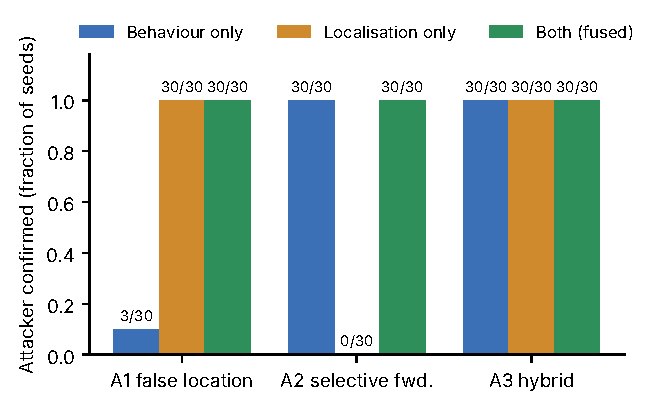
\includegraphics[width=0.78\textwidth]{fig2_coverage}
\caption{Evidence coverage over 30 seeds. Each single-evidence branch is
blind to the attack that produces no signature in its class; the three
behavioural confirmations of the A1 attacker occur at a lower rate than the
same branch confirms honest beacons.}
\label{fig:coverage}
\end{figure}

Table~\ref{tab:coverage} and Fig.~\ref{fig:coverage} report attacker
confirmation by evidence configuration. The inversion between the two
single-evidence rows admits a structural explanation. Under A1 the attacker
forwards honestly, so no behavioural quantity departs from its null
distribution. The delivered-throughput series of every A1 run is identical to
the clean-network run of the same seed, in all 30 seeds (Fig.~\ref{fig:tput}).
Behavioural evidence alone nevertheless confirmed the A1 attacker in 3 of 30
seeds. These confirmations carry no attack signal: on the clean network the
behavioural branch alone confirms honest beacons in 15 of 90 node-seeds (17\%),
a higher rate than its 10\% on the A1 attacker. Symmetrically, under A2 the
attacker advertises its true position, and localisation evidence alone
confirmed it in 0 of 30 seeds; it confirmed no honest beacon in any run of the
campaign.

A single-evidence detector therefore has a region of the attack space it
cannot observe, and an adversary who knows which evidence is collected may
choose to occupy it. This follows from what each evidence class can physically
observe, and no threshold setting changes it.

The scope of the claim is narrow. Table~\ref{tab:coverage} establishes that
collecting both classes covers both attacks. It does not establish that
Stouffer fusion is responsible: a disjunctive rule that thresholds each branch
independently and confirms on either would achieve the same result on A1 and
A2, because in each case one branch is far into its tail while the other is
silent. Fusion and disjunction separate only where both branches are weak
simultaneously. The coverage result is a result about evidence collection; the
fusion-rule question is taken up in Section~\ref{sec:sweep}.

\begin{figure}[!t]
\centering
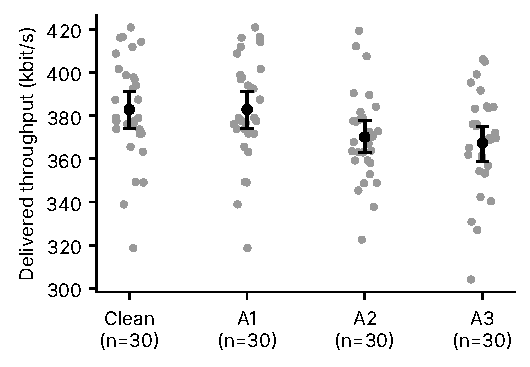
\includegraphics[width=0.6\textwidth]{fig3_throughput}
\caption{Delivered throughput by scenario, 30 seeds, with bootstrap 95\%
intervals of the mean. A1 and the clean network produce identical throughput
in every seed: the false-location attack has no packet-level footprint.}
\label{fig:tput}
\end{figure}

Two timing quantities are reported and must not be conflated. Detection
latency is the interval between attack onset and the first window in which the
attacker is confirmed. Isolation time is the timestamp of the first isolate
event written to the enforcement schedule. Over 30 seeds, the fused pipeline
confirmed the attacker in every seed of every attack. Median latency was
15.0\,s for A1 and A3 and 27.5\,s for A2 (means 20.0, 20.7 and 41.7\,s), with
a tail of slower confirmations reaching 80, 75 and 160\,s respectively.

The difference between attack classes is a property of the evidence, and the
model predicts its direction. Behavioural evidence reaches half confidence
weight at $n_{1/2} = 45$ observations against 5 for localisation
\eqref{eq:conf}. A2 is observable only through the behavioural branch, so its
confidence factor climbs an order of magnitude more slowly and confirmation
waits on the accumulation of transit packets. A1 and A3 are observable through
localisation, for which a handful of beacon receptions suffice. The constants were
fixed during calibration and not adjusted afterwards.

\subsection{Attack intensity and the fusion region}
\label{sec:region}

All three configurations confirm the A3 attacker in every seed, so the
experiment designed to show a fusion sensitivity advantage did not show one.
To locate where an advantage could appear we assume that branch anomaly
magnitude scales approximately linearly with attack intensity,
$A(f) \approx f A(1)$. For an RSSI-derived range residual under mobility, and
for a drop-rate statistic estimated from a finite window, that linearity is
plausible over a limited range but not guaranteed, so what follows locates the
region under an idealised model of the detector.

Let $\theta_B$ and $\theta_L$ be the intensities at which each branch alone
reaches the decision threshold, so that branch $X$ has anomaly
$\theta f/\theta_X$ at intensity $f$. With effective weights
$\tilde\omega_B, \tilde\omega_L$ the fused statistic of~\eqref{eq:stouffer}
crosses the threshold at
\begin{equation}
\label{eq:ffused}
f_F = \frac{\sqrt{\tilde\omega_B^{2} + \tilde\omega_L^{2}}}
           {\tilde\omega_B/\theta_B + \tilde\omega_L/\theta_L},
\end{equation}
and the family passes through a fusion-only region (an intensity at which
fusion confirms and neither branch does) precisely when
\begin{equation}
\label{eq:region}
f_F < \min(\theta_B, \theta_L).
\end{equation}
When the branches are equally sensitive the region is
$\theta_B/\sqrt2 < f < \theta_B$: a factor of $\sqrt2$ in intensity, half an
octave, and the widest it can be. Writing
$r = \max(\theta_B,\theta_L)/\min(\theta_B,\theta_L)$ for the sensitivity
ratio, \eqref{eq:region} with equal effective weights reduces to
\begin{equation}
\label{eq:ratio}
\frac{\sqrt{2}\,r}{1+r} < 1
\quad\Longleftrightarrow\quad
r < 1 + \sqrt{2} \approx 2.414 .
\end{equation}
With unequal weights, let $\tilde\omega_s$ weight the more sensitive branch and
$\tilde\omega_w$ the less sensitive one; the region exists if and only if
$r < \tilde\omega_w / \bigl(\sqrt{\tilde\omega_s^2 + \tilde\omega_w^2} -
\tilde\omega_s\bigr)$, which falls below $1+\sqrt{2}$ when the less sensitive
branch carries more weight (1.618 at twice the weight).

The condition concerns the attack family and not the detector, and the
distinction matters for how it is used. Write each branch's anomaly in units
of the decision threshold, $u = A_L/\theta$ and $v = A_B/\theta$, so that a
branch confirms alone when its coordinate reaches 1. With equal effective
weights the fused statistic confirms when $u + v \ge \sqrt2$, so the
fusion-only region is the triangle
\begin{equation}
\label{eq:wedge}
u < 1, \qquad v < 1, \qquad u + v > \sqrt2,
\end{equation}
which is non-empty for every equal-weight Stouffer detector, and with unequal
positive weights the corresponding region is non-empty as well. Every such
detector can therefore confirm attackers that neither branch confirms alone:
those whose two anomalies are each sub-threshold and of comparable normalised
size. Scaling an attack by intensity $f$ moves it along the ray
$(u, v) = f\,(1/\theta_L, 1/\theta_B)$ from the origin, and~\eqref{eq:ratio} is
the condition for that ray to pass through the triangle. A lopsided attack,
one that is much more visible to one branch than to the other, crosses the
more sensitive branch's threshold while the other branch's anomaly is still
too small to lift the fused statistic, and its ray misses the region. The ratio $r$ is therefore a property of how the
attack mixes the two misbehaviours, and it can be read from single-branch
detection curves for a given attack family before any fusion experiment is
run. Section~\ref{sec:sweep} tests it on two families that differ only in
that mix.

\subsection{False positives}
\label{sec:fp}

Over the 30-seed campaign the fused pipeline confirmed 9 of 90 honest
node-seeds on the clean network (10\%, Wilson 95\% interval 5.4--17.9\%) and 21
of 180 under attack (11.7\%, 7.8--17.2\%). The behavioural branch alone
confirmed 15 of 90 on the clean network and 35 of 180 under attack; the
localisation branch alone confirmed none. False confirmations are therefore a
property of the behavioural branch, whose peer-relative score fires whenever a
beacon's forwarding departs from its contemporaneous neighbours for benign
reasons such as mobility. Fusion with a silent localisation branch damps
these confirmations without removing them. With three monitored beacons per run, one false
positive moves per-run accuracy by 33 percentage points, which is why we
report counts instead of accuracy.

\subsection{Attack-intensity sweeps}
\label{sec:sweep}

We tested the fusion condition directly with two sweeps of the hybrid attack.
The primary sweep scales displacement and drop probability together from the
full-intensity A3 configuration over eleven levels, ten seeds each (110 runs,
Table~\ref{tab:sweep}). The second repeats eight levels with the drop
probability halved relative to displacement (80 runs, Table~\ref{tab:sweep2}).
Fig.~\ref{fig:sweep} shows both.

\begin{figure}[!t]
\centering
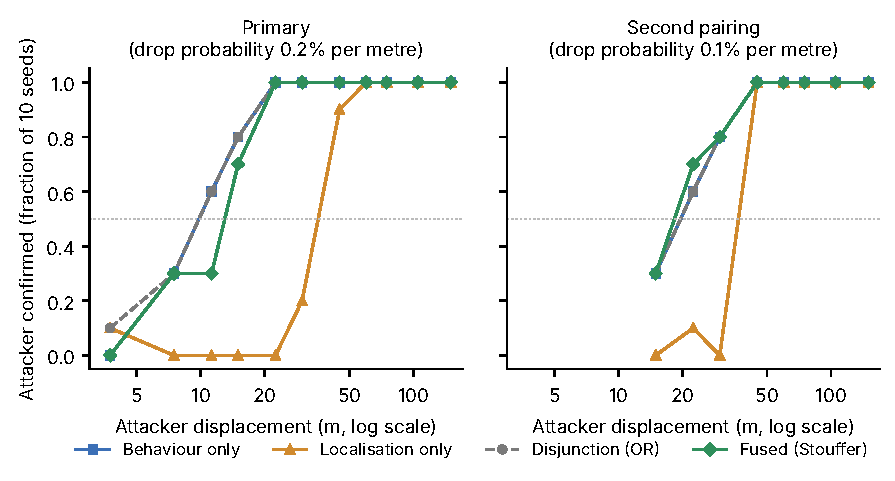
\includegraphics[width=\textwidth]{fig4_sweep}
\caption{Attacker detection across the two intensity sweeps, ten seeds per
point. Left: the branches' 50\% thresholds lie a factor of 3.63 apart, beyond the
$1+\sqrt2$ bound, and fusion falls below the disjunctive rule near the
behavioural threshold. Right: halving the drop rate moves the behavioural
curve and brings the ratio to 1.87, inside the bound, and fusion matches or
exceeds disjunction.}
\label{fig:sweep}
\end{figure}

\begin{table}[!t]
\caption{Primary sweep: attacker confirmed (of 10 seeds). Displacement is the
measured mean over the attacker's beacons after onset; below 45\,m it equals
the nominal $f\delta/2$ because the field boundary never clamps the offset.
Drop probability is $0.3f$. OR is the disjunctive rule over the
two single-evidence branches. FP counts honest beacons confirmed, of 20
node-seeds.}
\label{tab:sweep}
\centering
\small
\setlength{\tabcolsep}{4pt}
\begin{tabular}{@{}rrrrrrrr@{}}
\toprule
$f$ & Displ.\ (m) & Drop & Beh. & Loc. & OR & Fused & FP (OR / fused) \\
\midrule
0.025 & 3.75 & 0.0075 & 0 & 1 & 1 & 0 & 3 / 3 \\
0.05 & 7.5 & 0.015 & 3 & 0 & 3 & 3 & 5 / 4 \\
0.075 & 11.25 & 0.0225 & 6 & 0 & 6 & \textbf{3} & 1 / 1 \\
0.10 & 15.0 & 0.03 & 8 & 0 & 8 & \textbf{7} & 5 / 4 \\
0.15 & 22.5 & 0.045 & 10 & 0 & 10 & 10 & 5 / 5 \\
0.20 & 30.0 & 0.06 & 10 & 2 & 10 & 10 & 4 / 1 \\
0.30 & 45.0 & 0.09 & 10 & 9 & 10 & 10 & 4 / 4 \\
0.40 & 60.0 & 0.12 & 10 & 10 & 10 & 10 & 2 / 2 \\
0.50 & 74.9 & 0.15 & 10 & 10 & 10 & 10 & 3 / 2 \\
0.70 & 104.5 & 0.21 & 10 & 10 & 10 & 10 & 3 / 1 \\
1.00 & 147.1 & 0.30 & 10 & 10 & 10 & 10 & 3 / 3 \\
\bottomrule
\end{tabular}
\end{table}

\begin{table}[!t]
\caption{Second pairing: attacker confirmed (of 10 seeds) with drop probability
$0.15f$, half the rate of Table~\ref{tab:sweep}, at the same displacement.}
\label{tab:sweep2}
\centering
\small
\setlength{\tabcolsep}{4pt}
\begin{tabular}{@{}rrrrrrrr@{}}
\toprule
$f$ & Displ.\ (m) & Drop & Beh. & Loc. & OR & Fused & FP (OR / fused) \\
\midrule
0.10 & 15.0 & 0.015 & 3 & 0 & 3 & 3 & 5 / 4 \\
0.15 & 22.5 & 0.0225 & 6 & 1 & 6 & \textbf{7} & 1 / 1 \\
0.20 & 30.0 & 0.03 & 8 & 0 & 8 & 8 & 5 / 4 \\
0.30 & 45.0 & 0.045 & 10 & 10 & 10 & 10 & 5 / 5 \\
0.40 & 60.0 & 0.06 & 10 & 10 & 10 & 10 & 4 / 1 \\
0.50 & 74.9 & 0.075 & 10 & 10 & 10 & 10 & 2 / 2 \\
0.70 & 104.4 & 0.105 & 10 & 10 & 10 & 10 & 3 / 2 \\
1.00 & 147.1 & 0.15 & 10 & 10 & 10 & 10 & 3 / 2 \\
\bottomrule
\end{tabular}
\end{table}

\subsubsection{Primary sweep: the attack path misses the fusion-only region}

Behavioural detection falls from 8 of 10 at 15\,m to 6, 3 and 0 of 10 at 11.25,
7.5 and 3.75\,m; it reaches half detection at $\theta_B = 9.8$\,m, interpolated
on log intensity. Localisation evidence reaches half detection at
$\theta_L = 35.7$\,m. The measured ratio is $r = 3.63$. Resampling each level's
ten seeds as independent Bernoulli trials gives a bootstrap 95\% interval of
[2.67, 5.47], and fewer than 0.5\% of resamples fall below $1+\sqrt2$. Since
the less sensitive branch, localisation, carries the larger effective weight
through~\eqref{eq:conf}, the applicable bound is tighter still. This attack
family's path does not enter the fusion-only region.

The sweep shows the consequence the bound predicts. Where the behavioural
branch is near its threshold, adding the weaker localisation branch dilutes
it: at 11.25\,m fusion confirmed the attacker in 3 of 10 seeds against 6 for
the disjunctive rule, and at 15\,m in 7 against 8; at every stronger intensity
both confirmed it in all ten. The mechanism is visible at seed level. Where the
behavioural branch is anomalous and the localisation branch sits at its null,
equal-weight Stouffer combination computes $(A_B + 0)/\sqrt2$, attenuating a
live branch by 29\%, because a branch with adequate sample count carries
confidence weight whether or not it carries signal. Disjunction is immune,
since it never mixes the two. The same attenuation works in the opposite
direction for honest beacons: a benign behavioural deviation that would cross
the threshold alone is also scaled by $1/\sqrt2$ when the localisation branch
is at its null. Equal-weight fusion therefore trades sensitivity near the
threshold for suppression of single-branch false alarms. Sections~\ref{sec:fp},
\ref{sec:sparse} and~\ref{sec:scale} measure the second side of that trade.

\subsubsection{Second pairing: the condition predicts the outcome}

The ratio depends on how the sweep couples the two intensities, and the second
sweep tests whether~\eqref{eq:ratio} predicts the consequence. The behavioural
curve moved exactly as drop probability dictates: 3, 6 and 8 of 10 at drops of
1.5, 2.25 and 3\% in both sweeps, so behavioural detection depends on the drop
rate alone. Localisation, which depends on displacement alone, stayed close
to its primary-sweep value, at $\theta_L = 36.7$\,m. With $\theta_B = 19.7$\,m the ratio falls to $r = 1.87$
(bootstrap 95\% interval [1.41, 2.21]), inside the equal-weight bound in every
resample.

The outcome changed as the condition predicts. Fusion never confirmed fewer
attackers than the disjunctive rule. At $f = 0.15$, at which the behavioural
branch alone confirmed 6 of 10, fusion confirmed 7: one seed in which neither
branch crossed its threshold but their combined evidence did. One seed is weak
evidence and we do not report it as a fusion benefit. What the two sweeps
establish is that the same detector dilutes or helps depending on how the
attack family mixes its two misbehaviours, and that the ratio predicting which
can be measured before fusion is applied. The effective weights vary by window
through~\eqref{eq:conf}; if localisation carries twice the weight of behaviour,
the bound tightens to 1.618, which 17\% of resamples satisfy.

Taken together with Table~\ref{tab:coverage}, the finding is that evidence
collection determines coverage, and whether the combination rule adds anything
against a given attack family is decided by the branches' relative
sensitivity to that family.

\subsection{Comparison with literature baselines}
\label{sec:baselines}

Table~\ref{tab:baselines} compares the pipeline with the baselines of
Section~\ref{sec:baselinedef} on identical traces. The pipeline's false
isolation is that of policy E$'$, since the baselines also isolate on their
own detection and, like E$'$ in practice, do not release.

\begin{table}[!t]
\caption{Pipeline against literature baselines on identical traces. Detection
counts the attacker isolated after onset; FI is honest beacons isolated on the
clean network; $\bar\Phi$ is clean-network false isolation (E$'$ for the
pipeline); latency is the median time from onset to isolation, in seconds,
for A1 / A2 / A3, given only where the attacker was detected in at least half
the seeds. 30 seeds at 0\,dB and 20 under shadowing.}
\label{tab:baselines}
\centering
\small
\setlength{\tabcolsep}{3.5pt}
\begin{tabular}{@{}llcccccc@{}}
\toprule
$\sigma_{sh}$ & Method & A1 & A2 & A3 & FI & $\bar\Phi$ & Latency A1 / A2 / A3 \\
\midrule
0\,dB & LND & 30/30 & 2/30 & 30/30 & 3/90 & 0.003 & 10 / -- / 15 \\
      & WD & 1/30 & 30/30 & 30/30 & 4/90 & 0.031 & -- / 20 / 40 \\
      & LND+WD & 30/30 & 30/30 & 30/30 & 7/90 & 0.034 & 10 / 20 / 15 \\
      & Pipeline & 30/30 & 30/30 & 30/30 & 9/90 & 0.050 & 15 / 27.5 / 15 \\
4\,dB & LND & 20/20 & 1/20 & 20/20 & 2/60 & 0.005 & 15 / -- / 22.5 \\
      & WD & 4/20 & 20/20 & 13/20 & 7/60 & 0.050 & -- / 60 / 270 \\
      & LND+WD & 20/20 & 20/20 & 20/20 & 8/60 & 0.054 & 15 / 60 / 22.5 \\
      & Pipeline & 20/20 & 20/20 & 20/20 & 6/60 & 0.045 & 15 / 125 / 20 \\
8\,dB & LND & 20/20 & 0/20 & 20/20 & 1/60 & 0.000 & 20 / -- / 65 \\
      & WD & 0/20 & 20/20 & 3/20 & 0/60 & 0.000 & -- / 120 / -- \\
      & LND+WD & 20/20 & 20/20 & 20/20 & 1/60 & 0.000 & 20 / 120 / 65 \\
      & Pipeline & 20/20 & 20/20 & 19/20 & 0/60 & 0.000 & 22.5 / 150 / 155 \\
\bottomrule
\end{tabular}
\end{table}

The single-evidence baselines reproduce the coverage result with detectors
we did not design. The localisation-only detector revoked the A1 and A3
attackers in every seed of every channel and the A2 attacker in at most 2 of
30, and those few revocations came at least 225\,s after onset, at about the
rate at which it revoked honest beacons. The behaviour-only detector isolated
the A2 attacker in every seed and the A1 attacker in at most 4 of 20. Each
literature family is blind to the attack outside its evidence class, as
Table~\ref{tab:families} predicts from published descriptions.

The disjunction of the two baselines is the more instructive comparison, and
on it the pipeline does not win. LND+WD covered every attack in every channel
with false isolation statistically indistinguishable from the pipeline's: the
paired difference in clean-network $\Phi$ (pipeline minus LND+WD) was 19
node-seconds at 0\,dB (95\% CI $[-22, 61]$) and $-10$ at 4\,dB ($[-62, 43]$),
and both were zero at 8\,dB. It isolated attackers as fast or faster. The
pipeline was slower by a mean of 3.7\,s on A1 at 0\,dB (CI $[2.0, 5.2]$), by
60\,s on A2 at 4\,dB ($[18, 104]$) and by 77\,s on A3 at 8\,dB ($[33, 122]$),
and no paired interval showed it faster.

This is what Section~\ref{sec:region} predicts. A1 and A2 each disturb one
branch only, and A3 at its evaluated intensity lies above both branches'
individual thresholds rather than in the fusion-only region, so for every
attack evaluated here a disjunction loses nothing to fusion and
avoids the attenuation of a live branch by a silent one. The latency gap is
largest under shadowing, plausibly because the pipeline's behavioural branch
also waits for its confidence weight to saturate, which a reputation
threshold does not. In this network, therefore, the pipeline's detection is
matched by two calibrated classical detectors run in parallel.
Sections~\ref{sec:sparse} and~\ref{sec:scale} show that this does not carry
over to a sparse or a larger network; there the same disjunction withdrew
11--24\% of honest-beacon service against 0--3\% for the pipeline.

\subsection{Isolation policy under attack}
\label{sec:policy}

Table~\ref{tab:policy} and Fig.~\ref{fig:recovery} report the enforced runs of
the original campaign, five seeds per cell, and Fig.~\ref{fig:firstiso} the time
of first isolation under each policy over the 30-seed campaign. Detection is
identical across policies within each attack: the policies differ only in what
follows a verdict.

\begin{table}[!t]
\caption{Isolation policy comparison in the enforced runs, five seeds per cell.
Times in seconds, means over seeds; the attack begins at $t = 30$\,s. Policy C performs no
isolation.}
\label{tab:policy}
\centering
\small
\begin{tabular}{@{}llccc@{}}
\toprule
Attack & Policy & Isolation time & $R_{TH}$ & Recovery time \\
\midrule
A1 & C & -- & 0.97 & -- \\
   & D & 20.0 & 0.92 & 5.2 \\
   & E & 45.0 & 0.95 & 44.8 \\
A2 & C & -- & 0.93 & -- \\
   & D & 20.0 & 0.94 & 6.2 \\
   & E & 54.0 & 0.90 & 25.6 \\
A3 & C & -- & 0.93 & -- \\
   & D & 20.0 & 0.95 & 4.2 \\
   & E & 45.0 & 0.94 & 35.0 \\
\bottomrule
\end{tabular}
\end{table}

\begin{figure}[!t]
\centering
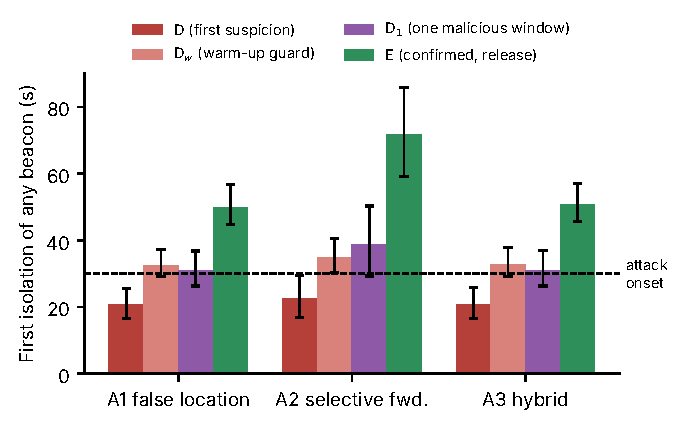
\includegraphics[width=0.78\textwidth]{fig5_first_isolation}
\caption{First isolation of any monitored beacon by policy, 30 seeds, with
bootstrap 95\% intervals. Policy D typically fires before the attack begins, so
what it first removes cannot be the attacker; D$_w$ and D$_1$ fire just after
onset, and E fires at onset plus detection latency.}
\label{fig:firstiso}
\end{figure}

Policy D first isolates at a median of 15\,s in every scenario, including the
clean network, before the attack begins at 30\,s. The 20.0\,s in
Table~\ref{tab:policy} is a five-seed mean (individual seeds 10--35\,s, median
20\,s), and is the same in all three attacks because the first isolation
precedes the attack and so depends only on the seed. The enforced runs used
the original campaign's calibration rather than the held-out seeds 101--105,
which moves one of the five seeds from 20 to 35\,s. What D removes at that point cannot be the
attacker. Its apparently fast recovery time of 4.2--6.2\,s is consequently an
artefact of having isolated before there was anything to recover from. D$_w$
and D$_1$ first isolate at medians of 30 and 35\,s. Policy E first isolates at
a median of 45\,s under A1 and A3 and 57.5\,s under A2, which is 30\,s plus the
corresponding detection latency: confirmation and enforcement coincide.

\begin{figure}[!t]
\centering
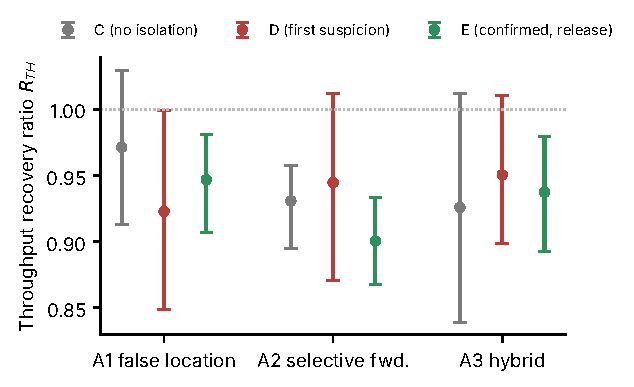
\includegraphics[width=0.68\textwidth]{fig6_recovery}
\caption{Throughput recovery ratio $R_{TH}$ in the enforced runs, five seeds,
with bootstrap 95\% intervals. The intervals exceed every between-policy
difference, so we claim no throughput advantage for any policy.}
\label{fig:recovery}
\end{figure}

Recovery ratios span 0.90--0.97 across all nine cells, with confidence intervals
substantially exceeding the differences between them (Fig.~\ref{fig:recovery}).
We claim no throughput advantage for any policy. Throughput debt, which we had
intended as a summary recovery metric, proved unusable: it returns non-zero
values on clean runs, because the baseline window is short relative to the
throughput variance of a mobile topology. Correcting it requires a later attack
start and a wider baseline window.

\subsection{Cumulative false isolation}
\label{sec:phi}

The comparison that separates the policies is not made under attack. On a clean
network every isolation is a false isolation, and $\Phi$ from~\eqref{eq:Phi} is
directly measurable. Table~\ref{tab:phivariants} and Fig.~\ref{fig:phi} report
it over 30 seeds for every policy, on the clean network and under each attack.

\begin{table}[!t]
\caption{Cumulative false isolation $\Phi$ (node-seconds) of honest beacons by
policy, 30 seeds. Honest isolated counts node-seeds; 95\% intervals are
percentile bootstrap over seeds. The final column is the paired difference from
policy E.}
\label{tab:phivariants}
\centering
\small
\setlength{\tabcolsep}{4pt}
\begin{tabular}{@{}llcrcc@{}}
\toprule
Network & Policy & Honest isolated & $\Phi$ & 95\% CI & $\Phi - \Phi_E$ [95\% CI] \\
\midrule
Clean & D     & 90/90 & 1052 & [1025, 1077] & 1005 [964, 1044] \\
      & D$_w$ & 90/90 & 1018 & [994, 1039]  & 971 [933, 1006] \\
      & D$_1$ & 88/90 & 897  & [843, 950]   & 851 [785, 911] \\
      & E     & 9/90  & 47   & [18, 79]     & -- \\
A1    & D$_1$ & 59/60 & 611  & [573, 648]   & 565 [519, 609] \\
      & E     & 8/60  & 47   & [18, 79]     & -- \\
A2    & D$_1$ & 58/60 & 587  & [532, 638]   & 557 [499, 612] \\
      & E     & 7/60  & 30   & [10, 54]     & -- \\
A3    & D$_1$ & 59/60 & 586  & [526, 639]   & 571 [514, 625] \\
      & E     & 6/60  & 15   & [2, 31]      & -- \\
\bottomrule
\end{tabular}
\end{table}

\begin{figure}[!t]
\centering
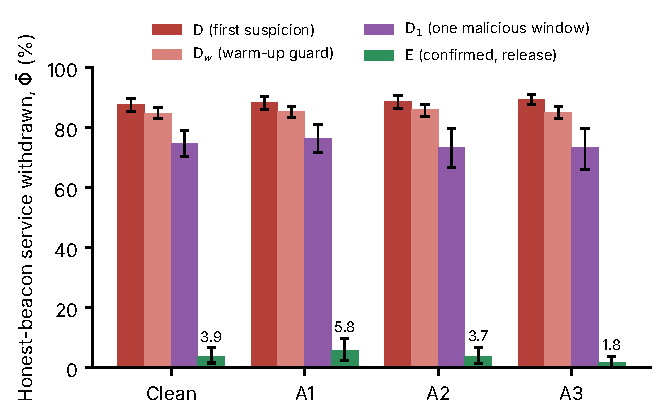
\includegraphics[width=0.8\textwidth]{fig8_phi}
\caption{Fraction of honest-beacon service withdrawn, $\bar\Phi$, by policy and
network, 30 seeds, with bootstrap 95\% intervals. Every immediate policy
withdraws 73--90\% of honest service; confirmation-gated isolation (E)
withdraws 2--6\%.}
\label{fig:phi}
\end{figure}

Policy D isolates on the first suspicious window, which typically falls before
any attacker is active. To test whether the comparison rests on a start-up
transient, D$_w$ ignores each beacon's first three usable windows, and D$_1$
isolates on the first window of malicious evidence without the persistence
requirement. On the clean network D$_w$ isolated all 90 honest node-seeds and
D$_1$ 88 of 90, with mean $\Phi$ of 1018 and 897 node-seconds against 47 for
policy E, which isolated 9 of 90. The paired difference between D$_1$ and E is
851 node-seconds (bootstrap 95\% CI [785, 911]); in normalised form D$_1$
withdraws 74.8\% of honest-beacon service and E 3.9\%. The advantage therefore
does not come from the start-up transient: removing the persistence requirement
alone is enough to isolate nearly every honest beacon. Under attack the same
ordering holds, and every paired interval excludes zero. Replaying the
original campaign's five clean seeds under that campaign's own calibration
gives D 1054 and E 49 node-seconds, inside the corresponding 30-seed
intervals. This checks the calibration and not the replay itself: both
figures are computed offline.

The replay itself was tested on clean seeds 1--10 by enforcing the replayed
schedules and rebuilding them from the verdicts issued under isolation
(Section~\ref{sec:method}). Isolation lowered $\Phi$ for both policies: D$_1$
from 910.5 to 829.5 node-seconds (paired difference $-81$, 95\% CI
$[-201.5, 45.5]$) and E from 32.5 to 24.5 (difference $-8$, CI $[-22, 0]$).
Neither interval excludes zero, and per seed the D$_1$ difference ranged from
$-370$ to $+295$, so the replay is unbiased within this resolution but noisy
for the immediate policy, and per-seed values of $\Phi$ for D$_1$ should not
be read individually. The comparison the paper rests on survived: under
isolation D$_1$ withdrew 69.1\% of honest-beacon service and E 2.0\%, D$_1$
exceeded E in all ten seeds, and the paired difference was 805 node-seconds
(CI $[693.5, 917]$) against 878 in the replay. For E the replay, if anything,
overstates $\Phi$.

The mechanism is that the policies inherit different bounds. Policy E isolates
only on confirmation, so its false-isolation rate is bounded by the detector's
false-confirmation rate of about 10\% (Section~\ref{sec:fp}). The immediate
policies isolate on weaker evidence, which on an uncontested network fires on
nearly every monitored beacon. The three-state verdict's contribution is the
tighter bound; it does not change what the detector can see.
Section~\ref{sec:release} shows that release contributes little to the gap.

The immediate policies are our own constructions, and the strongest of them,
D$_1$, isolates on a single window of evidence. Published schemes usually
wait for evidence to accumulate before they act: the localisation-only
baseline revokes a beacon only after more than $\tau'$ alerts, and the
behaviour-only baseline only after 20 packets of evidence. Both had low false
isolation in the dense network (0.3\% and 3.1\% of honest-beacon service,
Table~\ref{tab:baselines}). The comparison in Table~\ref{tab:phivariants} should
therefore be read as a measure of what acting before evidence accumulates
costs, not as a comparison with published practice. What the policies here
add is the size of that cost (about 75\% of honest-beacon service on a clean
network). Confirmation is one accumulation rule among several, and it was not
the cheapest in every network; Sections~\ref{sec:baselines},
\ref{sec:sparse} and~\ref{sec:scale} compare it with the two baselines.

\subsection{Release under isolation}
\label{sec:release}

The schedules above were built from verdicts issued while no beacon was
isolated. Re-verifying the enforced runs of the original campaign exposed a
behaviour that this construction hides. While a beacon is isolated it
forwards no transit traffic, so its behavioural branch falls below the
minimum sample: across the enforced runs behavioural evidence was usable in
1.6\% of the windows in which a beacon was isolated, against 54\% for the same
beacons and windows without isolation, while localisation evidence remained
usable in every window. For the A2 attacker, whose only signature is
behavioural, the fused trust therefore recovers once it is isolated. When the
E schedule was rebuilt from the verdicts issued under isolation, the A2
attacker was isolated at 45--65\,s and released at 115--160\,s in all five
seeds, after the twelve clean windows that clearing requires. A1 and A3
remained isolated, because their position lie keeps the localisation branch
in its tail. In a closed loop E would therefore cycle a forwarding attacker
between isolation and re-admission. Unlike timed redemption or an on--off
attack~\cite{bansal2003ocean,sun2006attacks}, this needs no timer and no
change in the attacker's behaviour. The replayed schedules contain milder
cases of the same effect: even without isolation, E released the attacker in
7 of the 90 attacked runs of the 30-seed campaign and in 3 of 60 at 4\,dB.

Policy E$'$ (Section~\ref{sec:framework}) releases a beacon confirmed on
behavioural evidence only when that evidence returns, which an isolated
beacon cannot supply. Its closed-loop schedule is therefore exact for those
beacons, which stay isolated, and follows the replay for beacons confirmed on
localisation alone. Table~\ref{tab:release} gives its cost.

\begin{table}[!t]
\caption{False isolation under evidence-aware release. $\bar\Phi$ is the
fraction of honest-beacon service withdrawn; E$'$ is evaluated as the closed
loop would run it. The last column is the paired difference D$_1 -$ E$'$ in
node-seconds with its bootstrap 95\% interval. 30 seeds at 0\,dB, 20 under
shadowing.}
\label{tab:release}
\centering
\small
\setlength{\tabcolsep}{4pt}
\begin{tabular}{@{}llcccc@{}}
\toprule
$\sigma_{sh}$ & Network & $\bar\Phi$ E & $\bar\Phi$ E$'$ & $\bar\Phi$ D$_1$ & D$_1 -$ E$'$ [95\% CI] \\
\midrule
0\,dB & Clean & 0.039 & 0.050 & 0.748 & 837 [773, 901] \\
      & A1    & 0.058 & 0.075 & 0.764 & 551 [500, 601] \\
      & A2    & 0.037 & 0.047 & 0.734 & 550 [486, 607] \\
      & A3    & 0.018 & 0.035 & 0.732 & 558 [497, 617] \\
4\,dB & Clean & 0.024 & 0.045 & 0.688 & 771 [677, 858] \\
      & A1    & 0.016 & 0.029 & 0.694 & 532 [475, 586] \\
      & A2    & 0.011 & 0.014 & 0.686 & 538 [482, 589] \\
      & A3    & 0.008 & 0.008 & 0.658 & 520 [445, 584] \\
8\,dB & Clean & 0.000 & 0.000 & 0.602 & 723 [656, 786] \\
      & A1    & 0.000 & 0.000 & 0.622 & 498 [452, 541] \\
      & A2    & 0.036 & 0.036 & 0.514 & 382 [321, 449] \\
      & A3    & 0.026 & 0.026 & 0.491 & 372 [298, 438] \\
\bottomrule
\end{tabular}
\end{table}

Evidence-aware release removed re-admission entirely: no attacker isolated
under E$'$ was released, in any of the 209 runs in which one was isolated. The
cost in false isolation was small. On the clean network $\bar\Phi$ rose from
3.9\% to 5.0\% (paired increase 13 node-seconds, 95\% CI [2, 28]), and E$'$
withdrew at most 7.5\% of honest-beacon service in any condition. The gap to
D$_1$ remained between 372 and 837 node-seconds, with every interval
excluding zero. The small cost has a simple cause: 46 of the 50 honest
beacons that E$'$ isolated across the three channels were never released, so
E$'$ amounts to near-permanent isolation on confirmation. Its advantage over
the immediate policies therefore comes from confirmation gating, not from
release. Release under E affected few honest beacons, and on the evidence
here a releasing policy is worth having only if it can distinguish recovered
evidence from absent evidence.

Iterating the loop confirmed both findings. Over three rounds on ten seeds,
E released the A2 attacker in every seed once its own enforced verdicts were
used: the fraction of post-onset time the attacker spent isolated fell from
0.88 in the first round to 0.23 in the second, and recovered only to 0.78 in
the third as the re-admitted attacker was confirmed again, the oscillation the
mechanism predicts. Under E$'$ the attacker was never released in any round
and spent 0.88 of the post-onset time isolated throughout. On the clean
network E$'$ was a fixed point from the first round in all ten seeds, with
$\Phi$ unchanged at 37 node-seconds, whereas E's $\Phi$ moved between rounds
(32.5, 24.5, 33.5) in two of the ten.

The A2 throughput and recovery rows of Table~\ref{tab:policy} were produced
by a schedule that never released the attacker. They are the rows E$'$ would
produce, not those of E in a closed loop.

\subsection{Robustness to shadowing}
\label{sec:shadow}

\begin{table}[!t]
\caption{Shadowing robustness, 20 seeds per cell. ``Confirmed'' is the fused
pipeline's attacker detections; latency is the median [interquartile range]
time from attack onset to confirmation, since the distributions are strongly
right-skewed; $\bar\Phi$ is the fraction of honest-beacon service withdrawn.
The $\sigma_{sh} = 0$ rows are the 30-seed campaign. In one 4\,dB seed the
beacon that later attacks was already falsely confirmed 5\,s before onset; in
the clean run of that seed the false confirmation cleared at 115\,s, but in
all three attack runs it persisted to the end, so the detection is counted.
Its latency is undefined and that seed is excluded from the latency columns.
It is also the single localisation confirmation of A2 at 4\,dB.}
\label{tab:shadow}
\centering
\small
\setlength{\tabcolsep}{4pt}
\begin{tabular}{@{}llccccc@{}}
\toprule
$\sigma_{sh}$ & Attack & Beh. & Loc. & Confirmed & Latency (s) & $\bar\Phi$ E / D$_1$ \\
\midrule
0\,dB & A1 & 3/30 & 30/30 & 30/30 & 15.0 [15.0--15.0] & 0.058 / 0.764 \\
      & A2 & 30/30 & 0/30 & 30/30 & 27.5 [15.0--52.5] & 0.037 / 0.734 \\
      & A3 & 30/30 & 30/30 & 30/30 & 15.0 [15.0--15.0] & 0.018 / 0.732 \\
      & Clean & -- & -- & -- & -- & 0.039 / 0.748 \\
4\,dB & A1 & 5/20 & 20/20 & 20/20 & 15.0 [15.0--15.0] & 0.016 / 0.694 \\
      & A2 & 20/20 & 1/20 & 20/20 & 125.0 [57.5--212.5] & 0.011 / 0.686 \\
      & A3 & 20/20 & 20/20 & 20/20 & 20.0 [15.0--32.5] & 0.008 / 0.658 \\
      & Clean & -- & -- & -- & -- & 0.024 / 0.688 \\
8\,dB & A1 & 0/20 & 20/20 & 20/20 & 22.5 [20.0--40.0] & 0.000 / 0.622 \\
      & A2 & 20/20 & 3/20 & 20/20 & 150.0 [101.2--215.0] & 0.036 / 0.514 \\
      & A3 & 14/20 & 18/20 & 19/20 & 155.0 [70.0--212.5] & 0.026 / 0.491 \\
      & Clean & -- & -- & -- & -- & 0.000 / 0.602 \\
\bottomrule
\end{tabular}
\end{table}

\begin{figure}[!t]
\centering
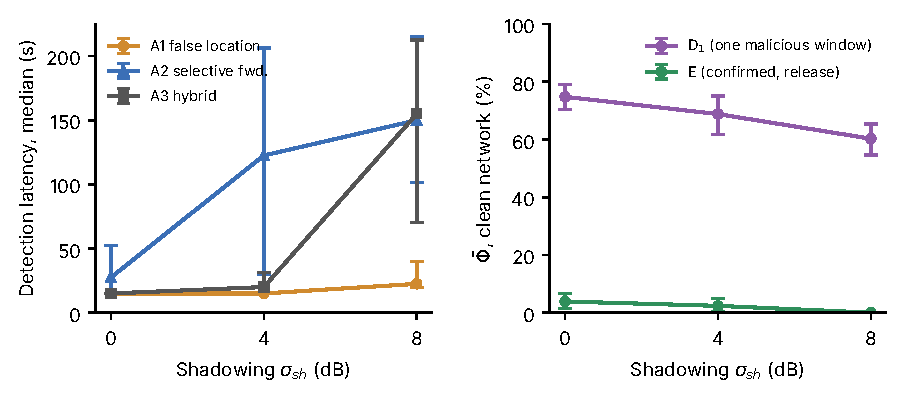
\includegraphics[width=\textwidth]{fig10_shadowing}
\caption{Effect of log-normal shadowing. Left: median detection latency, with interquartile range, rises sharply
for attacks seen through forwarding behaviour. Right: false isolation on the
clean network stays low for policy E and high for D$_1$.}
\label{fig:shadow}
\end{figure}

The campaign above uses a channel without shadowing, which flatters RSSI
ranging. We repeated it under log-normal shadowing with $\sigma_{sh} = 4$ and
8\,dB, 20 seeds per attack and channel. The pipeline was recalibrated on clean
runs of each channel, as a deployment would be; no threshold was changed.
Table~\ref{tab:shadow} and Fig.~\ref{fig:shadow} give the result.

Detection survived. The fused pipeline confirmed the attacker in every seed at
4\,dB and in 59 of 60 at 8\,dB, the miss being one A3 seed. The coverage
pattern held: localisation alone confirmed the A2 attacker in at most 3 of 20
seeds, and behaviour alone confirmed the A1 attacker in 5 of 20 at 4\,dB and
none at 8\,dB. Behavioural evidence degraded first: at 8\,dB it confirmed the
A3 attacker in 14 of 20 seeds, against 20 of 20 at 4\,dB. Shadowing adds link
loss that honest forwarders cannot control, which widens the peer distribution
the behavioural score is measured against.

The cost appeared as latency. Median time to confirmation for A2, the attack
visible only through forwarding, rose from 27.5\,s without shadowing to
125\,s at 4\,dB and 150\,s at 8\,dB; A3 rose to 155\,s at 8\,dB, once its
behavioural branch had degraded. A1, with its strong localisation signature,
was confirmed at a median of 15\,s at 4\,dB and 22.5\,s at 8\,dB.

False isolation did not grow. Policy E isolated at most 5 of 40 honest
node-seeds under attack and withdrew at most 3.6\% of honest-beacon service.
Recalibration widened the clean-network null enough that E isolated no honest
beacon in any clean 8\,dB seed. The immediate policies also isolated less as
the channel worsened, because the same widening raised their effective
threshold, but D$_1$ still withdrew 60--69\% of honest-beacon service on clean
networks, and the bootstrap intervals of D$_1$ and E did not overlap in any
condition.

\subsection{Sparse topology}
\label{sec:sparse}

Spreading the same 25 nodes over a $1000 \times 1000$\,m field changed the
balance of evidence. Behavioural evidence was usable in 18\% of windows,
against 52\% in the dense topology, while localisation evidence remained
usable in every window. Table~\ref{tab:sparse} gives the result.

\begin{table}[!t]
\caption{Sparse topology (25 nodes, $1000 \times 1000$\,m, 10 seeds).
Detection counts attackers isolated after onset (for the pipeline, confirmed);
latency is the median in seconds; FI and $\bar\Phi$ are for the clean network
(E$'$ for the pipeline). The single-branch rows count confirmations by each of
the pipeline's branches on its own. FI counts honest beacons isolated, except
for values marked $c$, which count honest beacons falsely confirmed by that
branch.}
\label{tab:sparse}
\centering
\small
\setlength{\tabcolsep}{4pt}
\begin{tabular}{@{}lccccc@{}}
\toprule
Method & A1 & A2 & A3 & FI & $\bar\Phi$ \\
\midrule
Pipeline & 10/10 & 4/10 & 10/10 & 0/30 & 0.000 \\
\quad latency & 62.5 & 132.5 & 62.5 & & \\
\quad behaviour branch only & 0/10 & 4/10 & 4/10 & 0/30$^{c}$ & -- \\
\quad localisation branch only & 10/10 & 0/10 & 10/10 & 0/30$^{c}$ & -- \\
LND & 10/10 & 0/10 & 10/10 & 0/30 & 0.000 \\
WD & 8/10 & 9/10 & 9/10 & 16/30 & 0.239 \\
LND+WD & 10/10 & 9/10 & 10/10 & 16/30 & 0.239 \\
Policy D$_1$ & & & & 8/30 & 0.100 \\
Policy D & & & & 30/30 & 0.849 \\
\bottomrule
\end{tabular}
\end{table}

The pipeline isolated no honest beacon in any sparse run, but it confirmed
the forwarding-only attacker in only 4 of 10 seeds and took a median of
62.5\,s to confirm the attacks with a localisation signature, four times the
dense figure. The cause is evidence scarcity: with few transit packets per
window the behavioural branch rarely reaches its minimum sample and its
confidence weight stays low. The behaviour-only reputation baseline, which
has no confidence weighting, isolated the A2 attacker in 9 of 10 seeds, but
on the clean network it also isolated 16 of 30 honest node-seeds and withdrew
23.9\% of honest-beacon service, because broken routes in a sparse network
look like dropped packets. The disjunction inherited both properties.

The single-branch rows locate the cause. The pipeline's own behavioural
branch, used alone, also confirmed no honest beacon, so fusion played no part
in the sparse result. What separates it from WD is how the behavioural
evidence is scored: against the beacon's neighbours in the same window, and
weighted by sample count. WD instead thresholds an absolute forwarding ratio.
The pipeline's behavioural branch therefore works as a peer-relative
behaviour-only detector, and in the sparse network it avoided the false isolation that the
absolute-ratio detector incurred, at the price of confirming the forwarding
attacker less often. The paired difference in clean-network $\Phi$ between the pipeline and LND+WD
was $-287$ node-seconds (95\% CI $[-446, -149]$), and the pipeline's $\Phi$
was lower under every attack as well (CIs excluding zero).

The comparison of Section~\ref{sec:baselines} therefore depends on the
topology. In the small dense network the disjunction matched the pipeline's
false isolation and was faster; in the sparse one it detected the forwarding
attacker more often but at roughly a quarter of honest-beacon service, which
is the trade $\Phi$ was introduced to expose. Section~\ref{sec:threats}
records a caveat on the sparse behavioural calibration.

\subsection{A larger network with two attackers}
\label{sec:scale}

Doubling the network to 50 nodes at the same density, with six monitored
beacons of which two attack simultaneously, left the main results in place
and sharpened the baseline comparison. Table~\ref{tab:scale} gives the
result.

\begin{table}[!t]
\caption{50-node network, two attackers, six monitored beacons, 10 seeds.
Detection counts runs in which both attackers were isolated after onset;
latency is the median over runs of the mean time to confirm the two
attackers, in seconds; FI and $\bar\Phi$ are for the clean network (E$'$ for
the pipeline). The single-branch rows count confirmations by each of the
pipeline's branches on its own. FI counts honest beacons isolated, except for
values marked $c$, which count honest beacons falsely confirmed by that
branch.}
\label{tab:scale}
\centering
\small
\setlength{\tabcolsep}{4pt}
\begin{tabular}{@{}lcccccc@{}}
\toprule
Method & A1 & A2 & A3 & Latency A1 / A2 / A3 & FI & $\bar\Phi$ \\
\midrule
Pipeline & 10/10 & 10/10 & 10/10 & 15 / 27.5 / 15 & 5/60 & 0.026 \\
\quad behaviour branch only & 0/10 & 10/10 & 10/10 & & 16/60$^{c}$ & -- \\
\quad localisation branch only & 10/10 & 0/10 & 10/10 & & 0/60$^{c}$ & -- \\
LND & 10/10 & 0/10 & 10/10 & 11.3 / -- / 17.5 & 2/60 & 0.005 \\
WD & 0/10 & 9/10 & 9/10 & -- / 20 / 67.5 & 7/60 & 0.108 \\
LND+WD & 9/10 & 9/10 & 9/10 & 12.5 / 20 / 15 & 9/60 & 0.113 \\
Policy D$_1$ & & & & & 60/60 & 0.742 \\
Policy D & & & & & 60/60 & 0.901 \\
\bottomrule
\end{tabular}
\end{table}

The pipeline confirmed both attackers in every attacked run, with medians of
15--27.5\,s, and isolated 5 of 60 honest node-seeds on the clean network.
Each single-evidence baseline was again blind outside its evidence class:
the localisation-only detector isolated no A2 attacker pair and the
behaviour-only detector no A1 pair. The coverage result therefore holds with
two simultaneous attackers and at twice the scale.

The disjunction of the baselines no longer matched the pipeline. It missed
one attacker in one run of each attack scenario, and its behavioural half
made it withdraw about four times as much honest-beacon service: 11.3\% on
the clean network against the pipeline's 2.6\%. Paired across
seeds, the pipeline's $\Phi$ was lower by 154 node-seconds under A2 (95\% CI
$[30, 277]$) and by 155 under A3 ($[42, 276]$); under A1 ($-163$,
$[-342, 8]$) and on the clean network ($-209$, $[-458, 0]$) the intervals
reached zero. Detection speed was indistinguishable: no paired latency
difference excluded zero. Immediate isolation was as costly as in the small
network, with D$_1$ withdrawing 72--74\% of honest-beacon service, and the
gap to E$'$ exceeded 1100 node-seconds under every scenario.

Here the cause is different from the sparse network. The pipeline's
behavioural branch alone falsely confirmed 16 of 60 honest node-seeds, more
than WD's 7, and the fused pipeline confirmed 5. The reduction from 16 to 5
is the attenuation of Section~\ref{sec:sweep} acting on honest beacons: a
benign behavioural deviation is scaled down by a localisation branch at its
null. Both counts come from the same topology and the same six-observer
median, so the observer count cannot explain the difference. At 50 nodes the
pipeline's lower $\Phi$ is therefore a benefit of fusion, and the dense
network shows the same effect on a smaller scale (15 of 90 honest node-seeds
for the behavioural branch alone against 9 fused).

Taken with Section~\ref{sec:sparse}, this bounds the baseline comparison of
Section~\ref{sec:baselines}. Only in the small dense network did two
classical detectors run side by side match the fused pipeline. In the sparse
network the advantage came from peer-relative scoring of behaviour, and at 50
nodes from fusion suppressing single-branch false alarms.


\section{Discussion}
\label{sec:discussion}

\subsection{Interpretation}

The coverage result is structural, following from what each evidence class can
physically observe rather than from a threshold setting, and it was obtained
with calibration held fixed across all scenarios. The implication for the
literature is narrow but practical. An accuracy reported against
localisation-visible attacks is an accuracy over that subset of the attack
space. EMBN-MANET's threat model is confined to false-location behaviour by
design, so its figure is correct within its scope and we do not dispute it.
What we would ask of any such report is one additional line: which attack
classes the evidence can observe at all.

The isolation result is the paper's strongest. Over 30 seeds,
confirmation-gated isolation withdrew 3.9\% of honest-beacon service on an
uncontested network (5.0\% with evidence-aware release) against 74.8\% for
the strongest immediate policy, with every paired interval excluding zero; the
ordering held under attack, under shadowing and when the schedules were
enforced. With evidence-aware release, its cost is the time an attacker
remains active before confirmation: a median of 15\,s for attacks with a localisation
signature and 27.5\,s for selective forwarding, rising to medians of 125--155\,s for
forwarding attacks under shadowing. Whether that trade is favourable depends on
the prior probability of attack and on what a wrongly removed beacon costs the
network. Where attack is rare and beacon coverage sparse, gating is preferable,
since $\Phi$ accumulates continuously while attacker exposure is bounded by the
confirmation delay. That bound holds only if release cannot be triggered by
missing evidence: under plain E a forwarding attacker is re-admitted once its
isolation silences its behavioural branch. Release is as consequential a
decision as isolation, and in our data the safe release rule made isolation on
confirmation close to permanent. Where attack is frequent and beacon redundancy high,
immediate isolation may be preferable. We present the trade rather than a
winner, and suggest that $\Phi$ or a comparable measure be reported routinely:
a mechanism's false-positive rate says nothing about how long its errors
persist.

\subsection{Limits of the evidence}

Whether fusion helped was decided by the attack family, not by the
combination rule. In the primary sweep the branches' sensitivity ratio was 3.63, beyond the
bound of 2.414, and Stouffer combination confirmed fewer attackers than a
disjunctive rule at the two intensities nearest the behavioural threshold.
Halving the drop rate relative to displacement brought the ratio to 1.87,
inside the bound, and fusion then never confirmed fewer and confirmed one more.
The detector was the same in both sweeps; only the mix of displacement and
drop rate changed. Fusion contributes against attackers whose two
misbehaviours are comparably visible to the two branches, and against
lopsided ones a disjunctive rule does as well or better. The baseline
comparison is the same result at the level of whole detectors: in the small
dense network, two calibrated single-evidence detectors run in parallel
matched the fused pipeline on every attack evaluated and were faster under
shadowing. In the sparse and 50-node networks the behaviour-only detector's
false isolation rose to 11--24\% of honest-beacon service while the
pipeline's stayed at 0--3\%, plausibly because of its confidence weighting
and peer-relative scoring;
there the benefit of fusion appears in $\Phi$, not in detection. Branch sensitivity to
a given attack family can be measured before fusion is applied, and no system
we surveyed reports checking it. An adaptive adversary could exploit this by
concentrating its misbehaviour on one axis, which is a further reason to
keep a single-branch path to confirmation alongside the fused statistic.

The aggregation stage changed no verdict anywhere. It belongs in the framework
as an unevaluated robustness extension, not as a validated component: a system
using only direct per-observer trust would reproduce every reported finding.
It remains because our campaign barely samples the conditions it exists to
handle, namely observers who disagree, direct trust that is noisy, and
recommenders who lie.

Neither isolation policy produced a defensible throughput benefit. This may be
a property of a dense 25-node topology in which AODV finds alternative routes
readily; enforcing isolation in the sparse topology is the obvious next
experiment.
Multipath recovery schemes~\cite{sirajuddin2021tbsmr} and isolation studies in
related ad hoc settings~\cite{kavitha2019india,buksh2024trust} suggest the
effect may be topology-dependent. On the evidence we have, the claim that
isolation restores network performance is unsupported. Finally,
throughput-based evaluation of A1 measures nothing, since A1 has no
packet-level footprint; the appropriate metric for that attack class is
localisation error.

\section{Threats to Validity}
\label{sec:threats}

\textbf{Construct validity.} Behavioural monitoring is node-global rather than
per-observer, so indirect trust operates on a coarser behavioural signal than
the model specifies. This weakens the aggregation ablation: the null may
reflect the implementation rather than the design. $\Phi$ for the 30-seed
campaign is computed by applying each policy offline to the same verdict
stream, which assumes that an isolation does not change later verdicts. For
the never-releasing policies the first isolation time is exact and only later
isolations in the same run can be affected; for E the release times can be,
and Section~\ref{sec:release} shows that for forwarding attackers they are.
Enforcing the replayed schedules on ten clean seeds and rebuilding them from
the verdicts issued under isolation moved neither policy's $\Phi$ by an amount
distinguishable from zero and preserved the D$_1$--E gap in every seed
(Section~\ref{sec:phi}). Iterating the loop for three rounds left E$'$ at a
fixed point on every clean seed and never released an attacker, while E
re-admitted the A2 attacker in every seed. Iteration approximates an online
detector but is not one, and it covers E and E$'$ on two scenarios. E$'$ was evaluated from verdicts
issued before isolation; its schedule is exact for beacons confirmed on
behaviour, which it never releases, and inherits the replay assumption for
beacons confirmed on localisation alone. E$'$ was designed after the
enforced runs were examined, so its evaluation is not blind to that
finding.

\textbf{Internal validity.} The recovery baseline window is short relative to
throughput variance, which is why we exclude throughput debt. Detection
thresholds were calibrated on held-out clean runs and fixed, which avoids
tuning to the test scenarios but means no scenario received its optimal
operating point.

\textbf{External validity.} The primary channel has no shadowing, multipath or
obstruction model; the shadowing campaign shows that detection and the
false-isolation result survive 4--8\,dB, at a substantial cost in latency for
forwarding attacks. The campaign is otherwise narrow in five ways. Attackers
are non-colluding and non-adaptive. Mobility follows a synthetic model rather
than a trace. The topologies are a 25-node network in a dense and a sparse
field and a 50-node network at the dense field's density; the sparse and
50-node campaigns measured detection and false isolation but not the
throughput effect of enforced isolation, so the throughput nulls rest on the
small dense field alone. Larger networks were limited by memory: a 50-node
run needs about 3\,GB, and a 100-node configuration did not fit the hardware
available. Three monitored beacons per run, six at 50 nodes, make rate-based
metrics coarse. And
only the hybrid attack's intensity is swept. We do not claim the results
generalise beyond this configuration.

\textbf{Comparative validity.} The two literature baselines re-implement
the evidence class and decision rule of Liu--Ning--Du alert counting and of
watchdog/CONFIDANT reputation; they are not complete reimplementations of
those systems, and they use our simulator's node-global behavioural counters
and our residual. Their thresholds were set on calibration seeds by rules we
chose, and a different but equally defensible rule would move their operating
points. Policies D, D$_w$ and D$_1$ are our own constructions, reasonable
stand-ins for isolate-on-suspicion behaviour. The comparison against
EMBN-MANET itself remains analytical, resting on a reading of its evidence
class and threat model.

\textbf{Statistical conclusion validity.} Coverage, latency, false positives
and $\Phi$ rest on 30 seeds with held-out calibration and paired bootstrap
intervals. The throughput, recovery, localisation-error and ablation results
rest on the five seeds of the original campaign; no difference among the
continuous throughput measures is claimed. The sparse and 50-node campaigns use ten seeds each, so their paired
intervals are wide and two of the 50-node comparisons reach zero. The sweeps
use ten seeds per level,
so the one-seed fusion gain in the second pairing is reported as consistent
with the condition, not as a measured benefit.

\section{Conclusion}
\label{sec:conclusion}

We evaluated multi-evidence verification and confirmation-gated isolation of
malicious beacon nodes in a mobile ad hoc network across 780 ns-3 simulation
runs.

For the two attack classes evaluated, single-evidence detection is blind to
attacks outside its evidence class, and collecting both behavioural and
localisation evidence removes the observed blind spots. Confirmation-gated
isolation reduced cumulative false isolation of honest beacons to 3.9\% of
available service against 74.8\% for the strongest immediate-isolation policy
over 30 seeds, at a median cost of 15--27.5\,s of attacker activity after
onset, and the gap held when the schedules were enforced. Releasing a beacon
when its verdict clears re-admitted forwarding attackers, whose behavioural
evidence disappears while they are isolated; requiring that evidence to return
before release prevented every re-admission and raised false isolation only to
5.0\%. Both results held under 4 and 8\,dB shadowing, where the price moved to
latency: forwarding attacks took a median of 125--155\,s to confirm. Every weighted
Stouffer detector has a fusion-only region, but an attack family scaled in
intensity reaches it only when the branches' detection thresholds for that
family lie within a factor of $1+\sqrt2$, and across two sweeps that condition
predicted whether fusion diluted ($r = 3.63$) or matched and marginally
exceeded ($r = 1.87$) a disjunctive rule. Consistent with that condition, a
calibrated disjunction of localisation-only and behaviour-only literature
baselines matched the fused pipeline's coverage and false isolation and
isolated attackers as fast or faster in the small dense network. In the
sparse network the disjunction detected the forwarding attacker more often
but withdrew 24\% of honest-beacon service, against none for the pipeline,
and in a 50-node network with two attackers it withdrew 11\% against 3\%
while the pipeline confirmed every attacker. The trust aggregation layer changed
no verdict, and neither isolation policy produced a throughput difference
exceeding its confidence interval.

We report these outcomes together because the negative ones bound the positive
ones. In a literature where reported accuracies cluster above 95\%, the more
informative questions are which attacks a detector can see and how long its
mistakes last.

\subsection{Future work}
\label{sec:future}

\textbf{Complete baselines.} Full implementations of EMBN-MANET and of a
behavioural trust-routing scheme, including their response mechanisms, on the
same topology and traces.

\textbf{Scale and topology.} Networks of 100 nodes and more, enforced
isolation in sparse topologies where it can affect delivery, varied mobility
speeds, and colluding or adaptive attackers.

\textbf{Fusion-rule comparison.} Bounded rules (arithmetic and geometric mean),
calibrated statistical rules (Stouffer, Fisher, Dempster--Shafer) and learned
rules (regularised logistic regression, gradient-boosted trees) compared on
identical oriented evidence, in configurations chosen on both sides of the
bound~\eqref{eq:ratio}, with folds partitioned by seed.

\textbf{Aggregation in its intended regime.} Noisy observers, conflicting
observers and malicious recommenders, which is where indirect and historical
trust are designed to matter.

\textbf{Post-isolation localisation error.} Splitting localisation error at the
isolation timestamp would give direct evidence that isolation restores a
degraded service, which throughput cannot show for A1.

\textbf{Online closed-loop evaluation.} The policies here were evaluated by
replay, one-step enforcement and a three-round iterated loop. Running the detector inside the
simulator, so that each isolation and release feeds back into later
verdicts, would test E$'$ and the replay assumption directly, and would allow
probationary release, in which a released beacon is re-isolated on its first
malicious window.

\textbf{Faster behavioural confirmation under shadowing.} The latency cost of
forwarding attacks under shadowing comes from the behavioural branch's slow
confidence saturation and widened peer distribution; adaptive half-weights or
a second behavioural observable could reduce it.

\section*{Acknowledgements}

The authors thank the developers and maintainers of the ns-3 network
simulator~\cite{ns3}, whose simulator and AODV, IEEE 802.11 and propagation
models this study builds on, and the developers of the open-source Python
scientific stack used for the analysis.

\section*{Declarations}

\textbf{Funding.} No funding was received for this work.

\textbf{Competing interests.} The authors declare no competing interests.

\textbf{Author contributions.} A.V.\ designed and implemented the simulator,
verification pipeline and experiments, and drafted the manuscript. D.V.C.\
supervised the work, contributed to the experimental design and revised the
manuscript. Both authors read and approved the final version.

\textbf{Data and code availability.} Simulation sources, the analysis
pipeline, the scripts that run every campaign and regenerate every data
figure, and the result tables, per-window verdicts and isolation schedules
for every campaign are available at
\url{https://github.com/kraghu356/manet-beacon-trust}. The raw per-run
simulator traces are available from the corresponding author
on reasonable request. No third-party dataset was used: every data point in
this paper was generated by the authors' simulations.

\textbf{Ethics approval.} Not applicable. This study involves neither human
participants nor animals.


\bibliography{refs}
\end{document}
